\documentclass{beamer}
%
% Choose how your presentation looks.
%
% For more themes, color themes and font themes, see:
% http://deic.uab.es/~iblanes/beamer_gallery/index_by_theme.html
%
\mode<presentation>
{
  \usetheme{default}      % or try Darmstadt, Madrid, Warsaw, ...
  \usecolortheme{default} % or try albatross, beaver, crane, ...
  \usefonttheme{default}  % or try serif, structurebold, ...
  \setbeamertemplate{navigation symbols}{}
  \setbeamertemplate{caption}[numbered]
  \setbeamertemplate{footline}[frame number]
} 

\usepackage[english]{babel}
\usepackage[utf8x]{inputenc}
\usepackage{tikz}
\usetikzlibrary{shapes.geometric,arrows}
\usepackage{pgfplots} % For Tikz
% Package for adding comments add disable in [] to remove all comments
%\usepackage[]{todonotes}


\title[Performance Analysis of Source-Seeking Algorithms with Integral Quadratic Constraints]{Performance Analysis of Source-Seeking Algorithms with Integral Quadratic Constraints}
\author{Adwait Datar}
\institute{PhD Workshop, 2021\\Technical University of Hamburg}
\date{$11^{th}$ Sept, 2021}

\begin{document}

\begin{frame}	
  \titlepage
\end{frame}

% Uncomment these lines for an automatically generated outline.
%\begin{frame}{Outline}
%  \tableofcontents
%\end{frame}
%%%%%%%%%%%%%%%%%%%%%%%%%%%%%%%%%%%%%%%%%%%%%%%%%%%%%%%%%%%%%%%%%%%%%
\begin{frame}{Source-seeking Algorithms}
	\begin{figure}[!htb]
		\centering
		\begin{minipage}{.5\textwidth}
			\centering
			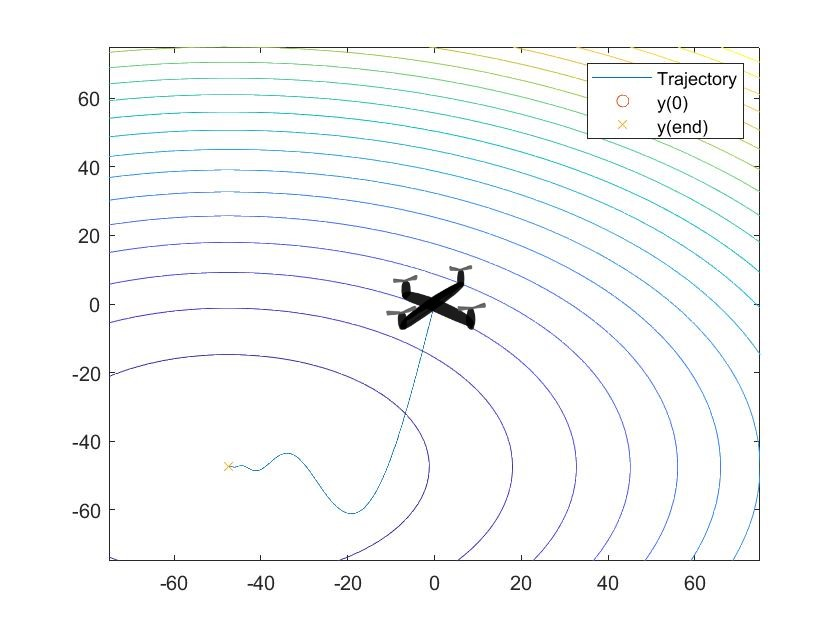
\includegraphics[width=0.9\linewidth,height=0.45\textheight]{figures/single_quad_field.jpg}
			\caption{Single quadrotor}
			\label{fig:single_quad}
		\end{minipage}%
		\begin{minipage}{0.5\textwidth}
			\centering
			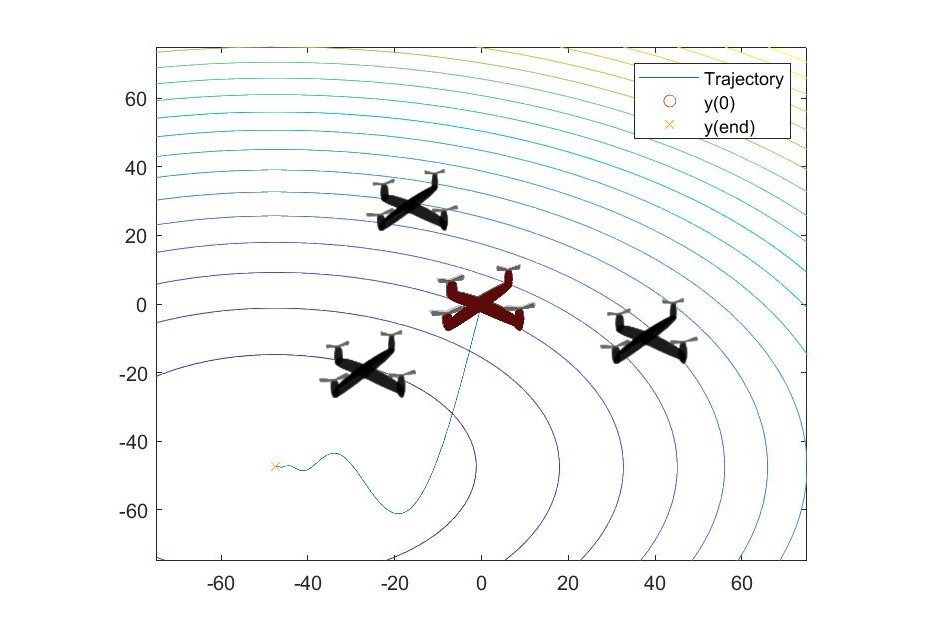
\includegraphics[width=\linewidth,height=0.45\textheight]{figures/multiple_quad_field.jpg}
			\caption{Multiple quadrotors}
			\label{fig:multiple_quads}
		\end{minipage}
		\end{figure}
	\begin{block}{Assumptions}
		\begin{itemize}		
			\item Field is differentiable (can be relaxed using sub-gradients) and convex
			\item Local gradients available at each agent (Replaced by gradient estimates in practise)
		\end{itemize}		
	\end{block}
\end{frame}
%%%%%%%%%%%%%%%%%%%%%%%%%%%%%%%%%%%%%%%%%%%%%%%%%%%%%%%%%%%%%%%%%%%%%
\begin{frame}{Motivations and relevant works}
	\begin{block}{Earlier work on analysis of source-seeking algorithms}
	\begin{itemize}
		\item Stability analysis but no performance guarantees [Attallah, 2020], [Datar, Paulsen and Werner, 2020]
		\item Lyapunov (storage) functions are constructed based on physically motivated energy like functions: Diagonal Lyapunov (storage) functions [Datar, Paulsen and Werner, 2020]
		\item Use small-gain arguments for general non-linear (LPV) agents [Attallah, Datar and Werner, 2020]
	\end{itemize}
	\end{block}	
	\begin{block}{Key contributions of this work}
	\begin{itemize}
		\item Performance analysis with guaranteed rates of convergence
		\item Quantifiable robustness w.r.t underlying field
		\item Less conservative results with dynamic non-causal multipliers
	\end{itemize}
\end{block}
\end{frame}
%%%%%%%%%%%%%%%%%%%%%%%%%%%%%%%%%%%%%%%%%%%%%%%%%%%%%%%%%%%%%%%%%%%%%
\begin{frame}{Control Architecture: Single Agent}
	\begin{figure}[!htb]
		\centering
		\begin{minipage}{.6\textwidth}
			\centering
			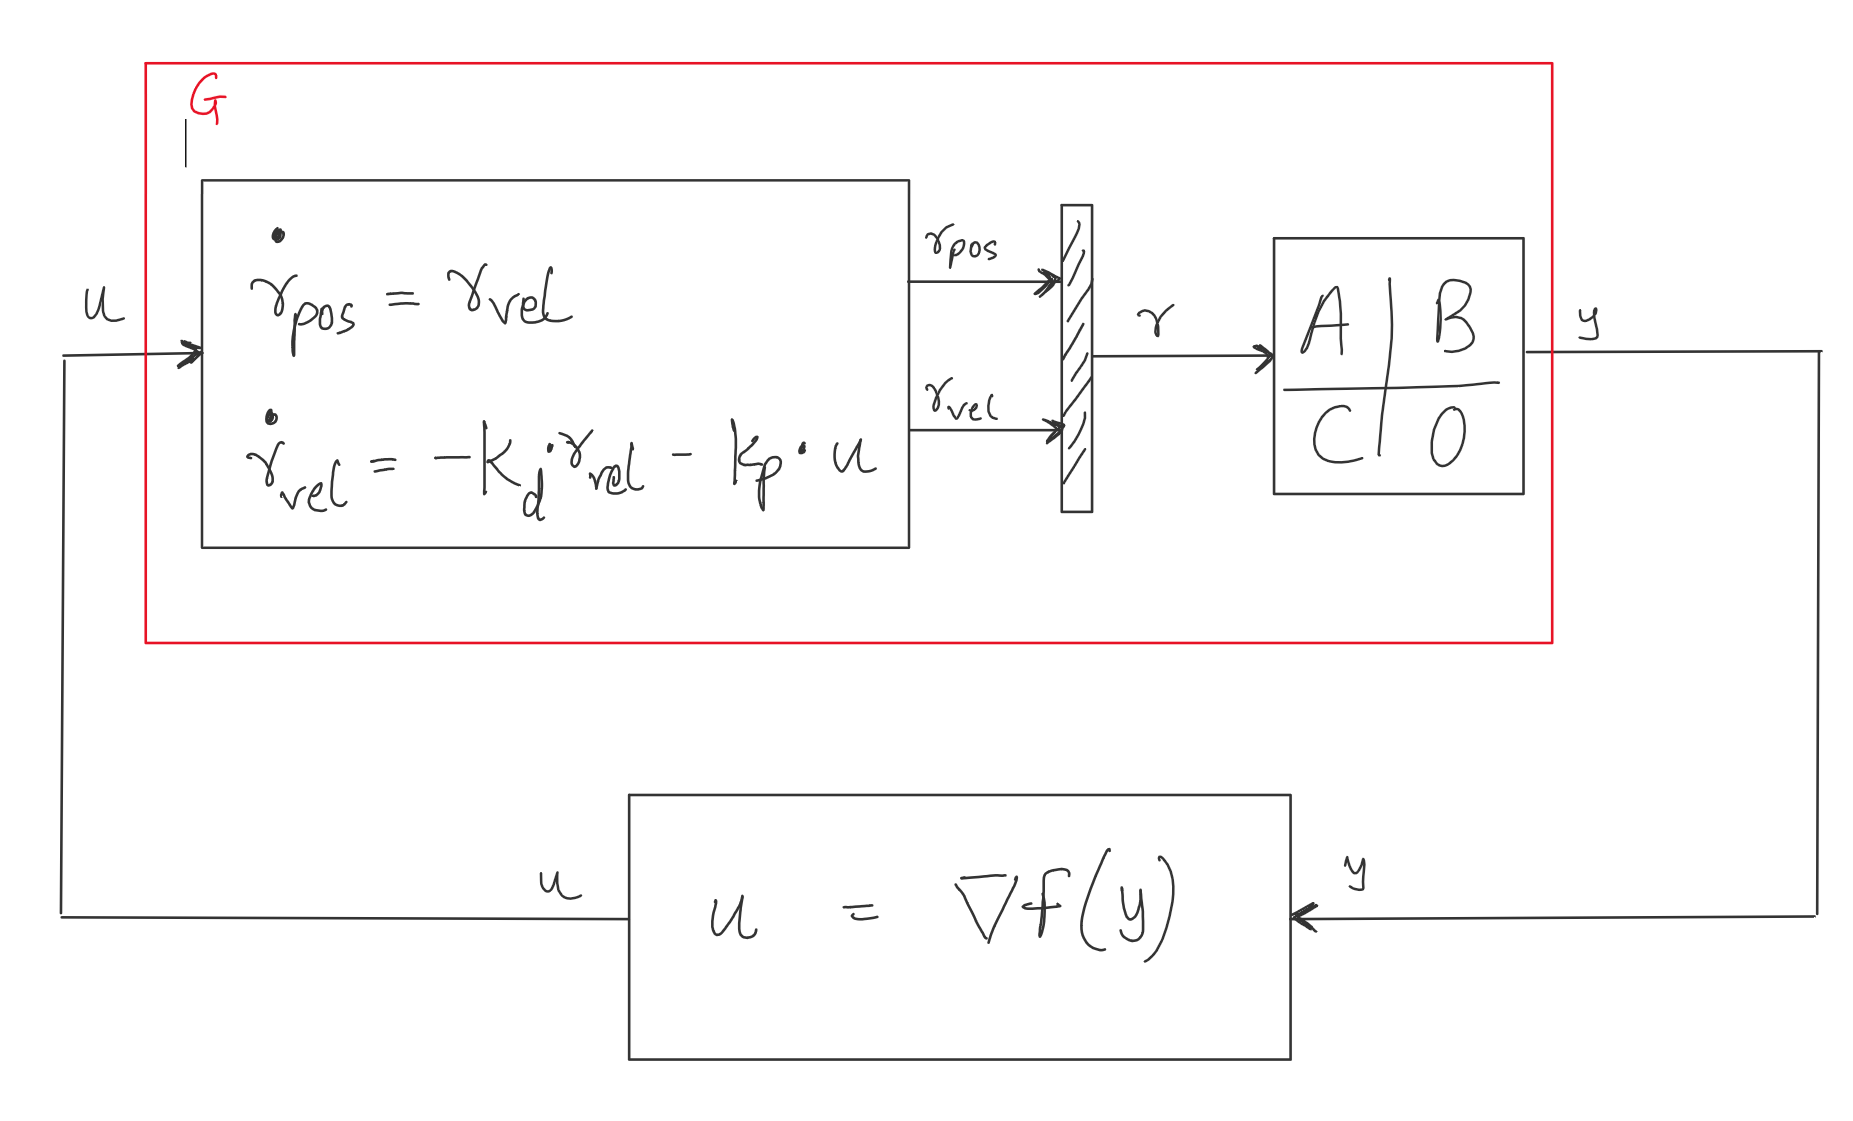
\includegraphics[width=6cm]{figures/Figure_IQC_paper.PNG}
			%\input{figures/quadrotor_trajectory}
			%\caption{Block diagram}
			\centering
			\label{fig:Figure_IQC_paper}
		\end{minipage}%
		\begin{minipage}{0.4\textwidth}
			\centering
			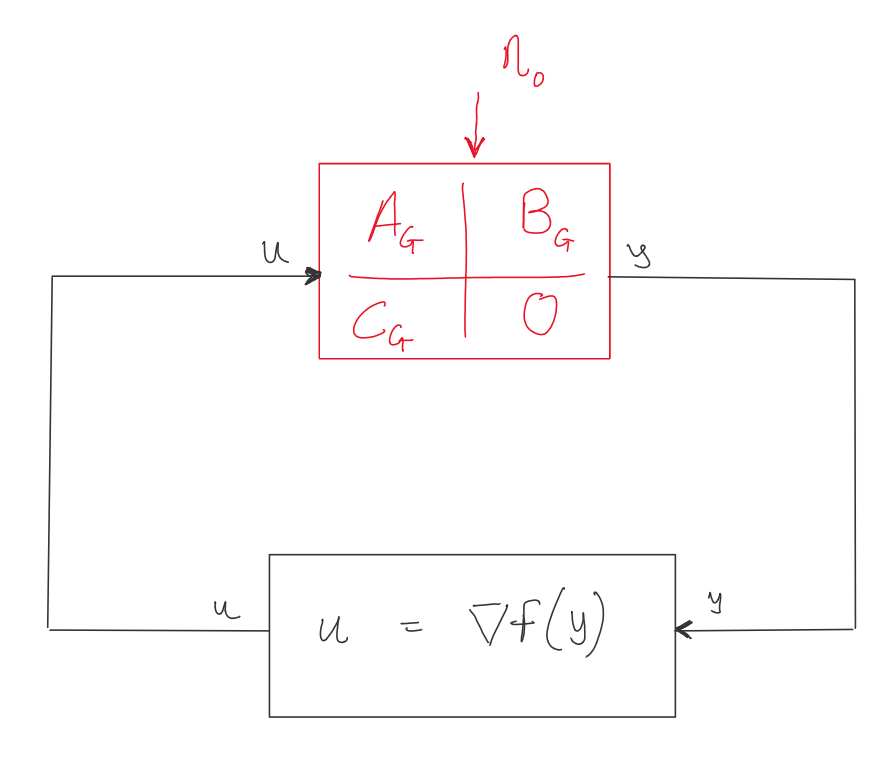
\includegraphics[width=1.1\linewidth,height=0.4\textheight]{figures/loop.png}
		%	\caption{Multiple quadrotors}
			%\label{fig:multiple_quads}
		\end{minipage}
	\end{figure}
%	\begin{figure}[t]
%		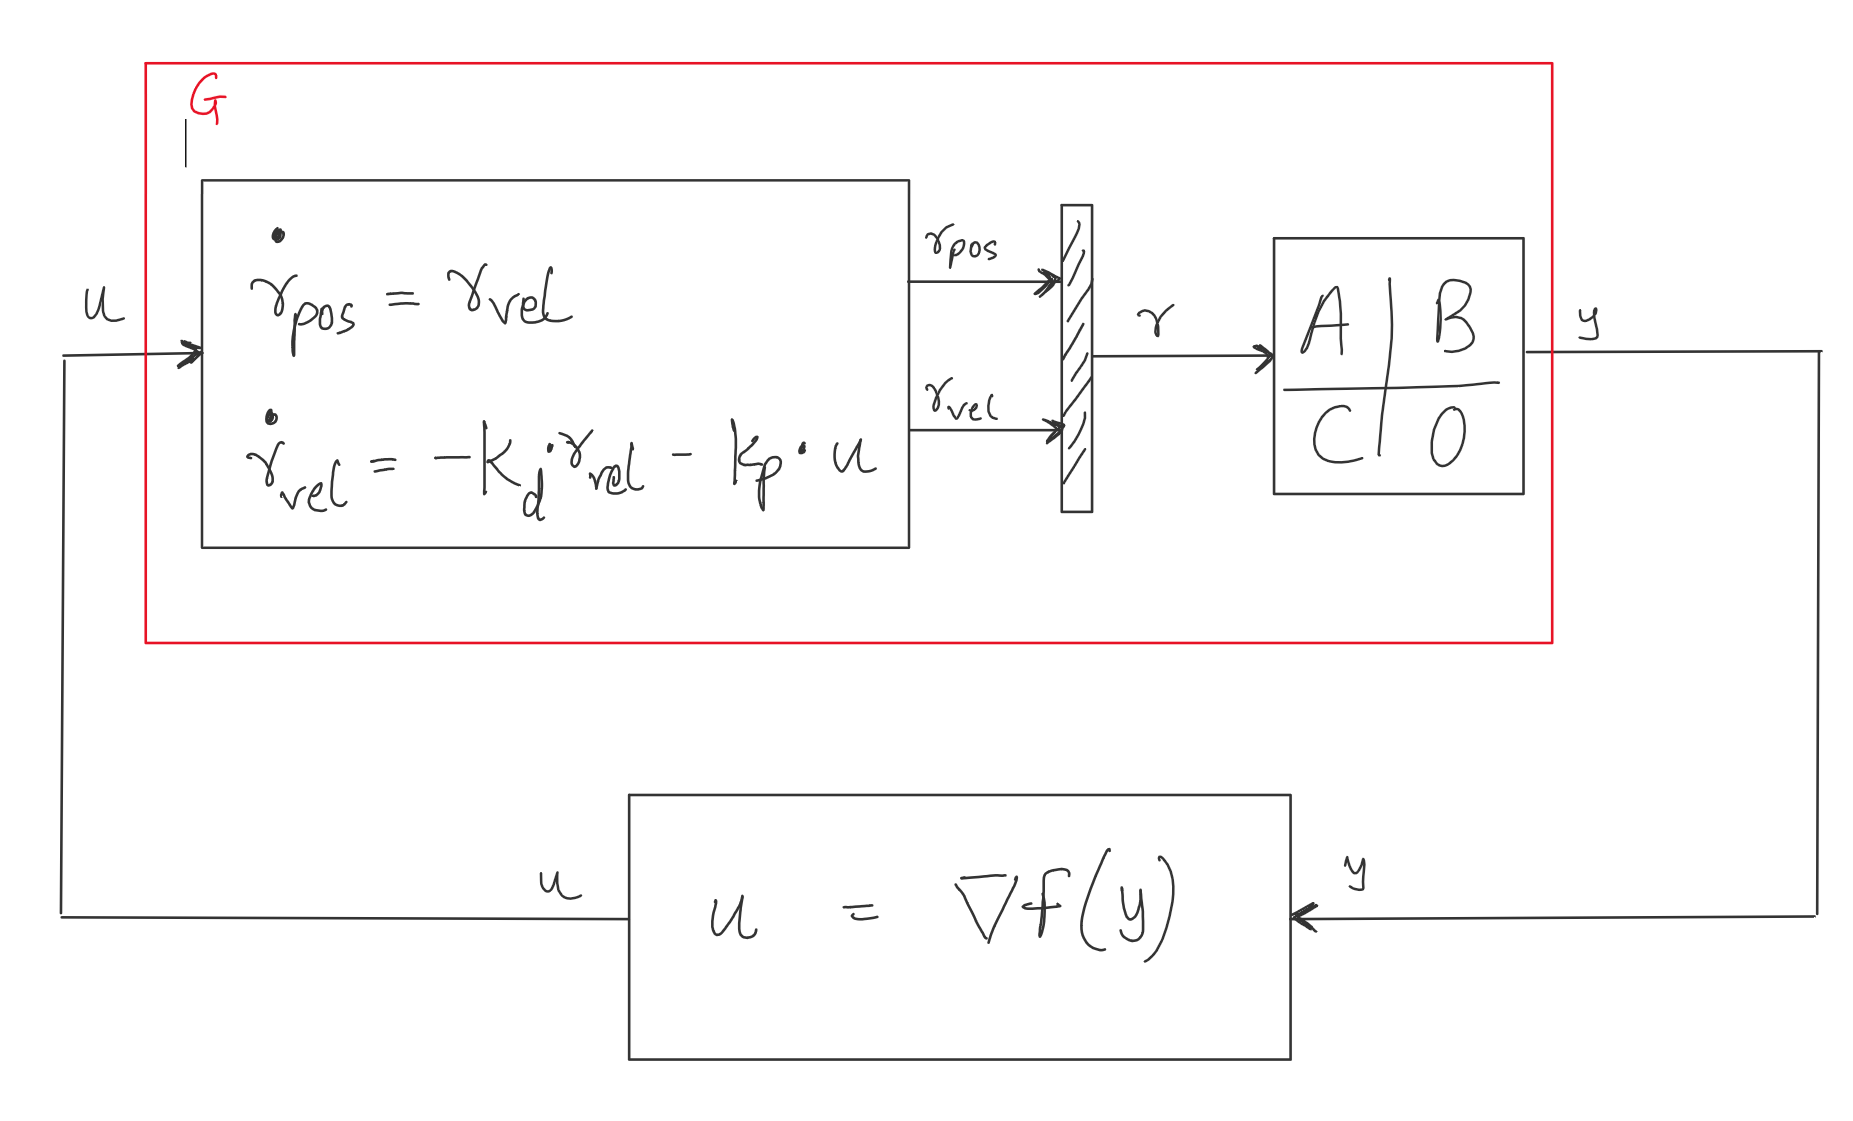
\includegraphics[width=8cm]{figures/Figure_IQC_paper.PNG}
%		%\input{figures/quadrotor_trajectory}
%		%\caption{Block diagram}
%		\centering
%		\label{fig:Figure_IQC_paper}
%	\end{figure}
	\begin{equation} \label{eq:sys_dyn_G}
		\begin{split}
			\Dot{\eta}(t)&=A_G\eta(t) + B_G u(t), \quad \quad \eta(0)=\eta_0\\
			y(t)&=C_G \eta(t) \\
			u(t)&=\nabla f(y(t)),
		\end{split}
	\end{equation}
\end{frame}
%%%%%%%%%%%%%%%%%%%%%%%%%%%%%%%%%%%%%%%%%%%%%%%%%%%%%%%%%%%%%%%%%%%%%
\begin{frame}{Decomposing flocking dynamics under quadratic fields}
	\begin{figure}[t]
		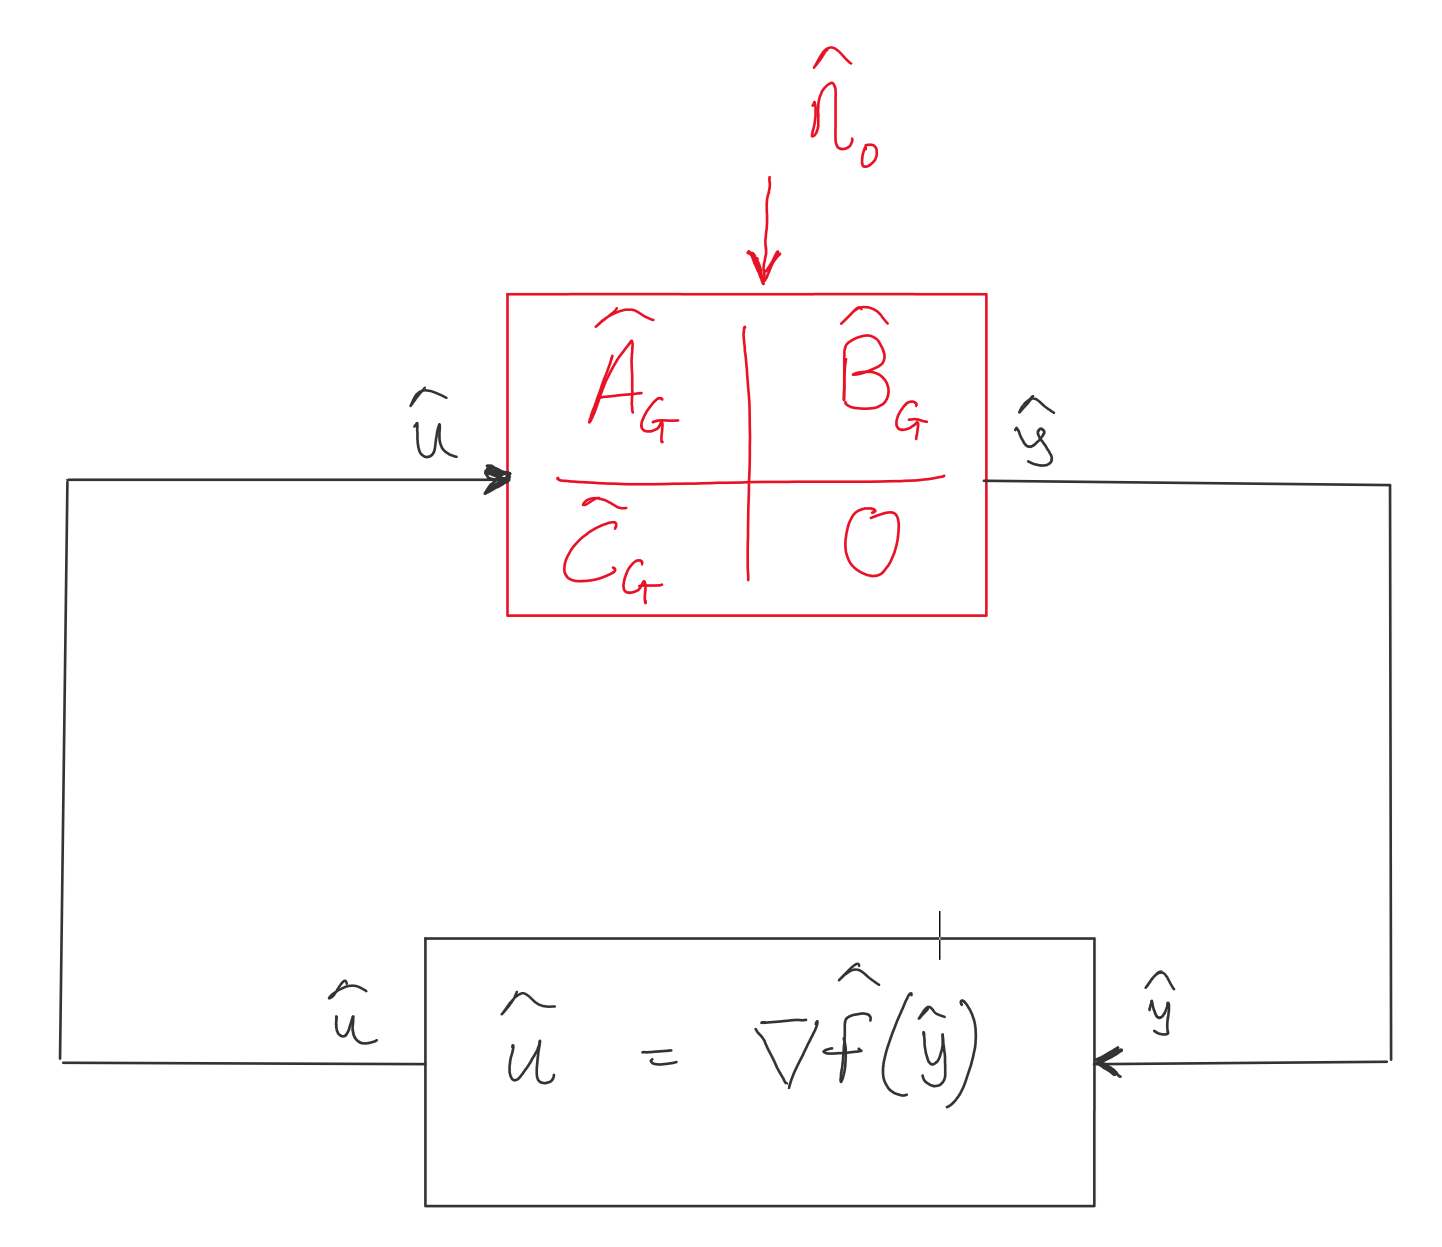
\includegraphics[width=6cm]{figures/loop_multiple_agents.PNG}
		%\input{figures/quadrotor_trajectory}
		\caption{Block diagram}
		\centering
		%\label{fig:Figure_IQC_paper}
	\end{figure}
	\begin{equation} \label{eq:flocking_dynamics}
		\begin{split}
			\Dot{\hat{\eta}}(t)&=(I_N \otimes A_G)\hat{\eta}(t) + (I_N \otimes B_G)\hat{u}(t),\\
			\hat{y}(t)&=(I_N \otimes C_G)\hat{\eta}(t) \\
			\hat{u}(t)&=\nabla \hat{f}(\hat{y}(t))-\nabla \mathcal{V}(\hat{y}(t))-(\mathcal{L}\otimes I_d)\Dot{\hat{y}}(t).
		\end{split}
	\end{equation}
\end{frame}
%%%%%%%%%%%%%%%%%%%%%%%%%%%%%%%%%%%%%%%%%%%%%%%%%%%%%%%%%%%%%%%%%%%%%
\begin{frame}{Decomposing flocking dynamics under quadratic fields}
	\begin{block}{Averaging out state, input and output:Center Of Mass(COM)} $\eta_c=\textnormal{avg}(\hat{\eta})$, $y_c=\textnormal{avg}(\hat{y})$, $u_c=\textnormal{avg}(\hat{u})$
	\end{block}
	\begin{block}{Quadratic fields (Linear gradients)}
	\begin{itemize}
	\item $f(y)=y^T Q y + c^Ty + d \implies \nabla f (y)=2 Qy + c$
	\item $\textnormal{avg}(\nabla \hat{f}(\hat{y}))=\nabla f (\textnormal{avg}(\hat{y}))=\nabla f(y_c)$
	\end{itemize}
	\end{block}
	\begin{block}{Averaging dynamics \eqref{eq:flocking_dynamics}}
	\begin{itemize}
		\item $\textnormal{avg}((I_N \otimes A_G)\hat{\eta})=A_G{\eta_c}$ (Similary for $B_G$ and $C_G$)
		\item $\textnormal{avg}(\nabla \mathcal{V}(\hat{y}))=\mathbf{0}$,$\textnormal{avg}((\mathcal{L}\otimes I_d))=\mathbf{0}$ 
	\end{itemize}
	\end{block}
	\begin{equation}\label{eq:COM_dynamics}
		\begin{split}
			\Dot{\eta_c}(t)
			% &=\frac{1}{N}(\mathbf{1}_N^T \otimes I_{n_\eta})((I_N \otimes A_G)\hat{\eta}(t) + (I_N \otimes B_G)\hat{u}(t)),\\
			% &=\frac{1}{N}(\mathbf{1}_N^T \otimes A_G)\hat{\eta}(t)+ \frac{1}{N}(\mathbf{1}_N^T \otimes B_G )\hat{u}(t)),\\
			&=A_G \eta_c + B_G u_c,\\
			\hat{y}_c(t)
			% &=\frac{1}{N}(\mathbf{1}_N^T \otimes I_{d})(I_N \otimes C_G)\hat{\eta}(t) \\
			&= C_G \eta_c\\
			\hat{u}_c(t)&=\nabla f (y_c).
		\end{split}
	\end{equation}
\end{frame}
%%%%%%%%%%%%%%%%%%%%%%%%%%%%%%%%%%%%%%%%%%%%%%%%%%%%%%%%%%%%%%%%%%%%%
\begin{frame}{Theory}
	\begin{block}{Relevant Literature}
		\begin{itemize}
			\item Exponential IQCs introduced in [Lessard,Recht and Packard, 2016], [Hu and Seiler, 2016], 
			\item Non-causal dynamic Zames Falb $\alpha$-IQCs [Freeman, 2018] 
			\item Parameterization of dynamics Zames Falb IQCs [Veenman and Scherer, 2018] 
		\end{itemize}
	\end{block}	
	\begin{block}{theoretical contribution of this work}
	\begin{itemize}
		\item Derivation of a general non-causal dynamic $\alpha$-ZF IQCs
		non-causal dynamic multipliers with an LMI-able parameterization
	\end{itemize}
\end{block}	
\end{frame}
%%%%%%%%%%%%%%%%%%%%%%%%%%%%%%%%%%%%%%%%%%%%%%%%%%%%%%%%%%%%%%%%%%%%%
\begin{frame}{Loop in the deviation variables}
	\begin{block}{Equilibrium}
		\begin{equation} \label{eq:sys_dyn_G_delta}
			\begin{split}
				0&=A_G\eta_* + B_G u_*=A_G\eta_*\\
				y&=C_G \eta_*\\
				u_*&=\nabla f(y_*)=0
			\end{split}
		\end{equation}
	\end{block}
	\begin{block}{Loop in the transformed variables}
		\begin{equation} \label{eq:sys_dyn_G_tilde}
			\begin{split}
				\Dot{\Tilde{\eta}}(t)&=A_G\Tilde{\eta}(t) + B_G \Tilde{u}(t), \quad \quad \Tilde{\eta}(0)=\eta_0-\eta_*\\
				\Tilde{y}(t)&=C_G \Tilde{\eta}(t)
			\end{split}
		\end{equation}
		and 
		\begin{equation} \label{eq:delta}
			\Tilde{u}(t)=\nabla f(\Tilde{y}(t)+y_*)
		\end{equation}
	\end{block}
\end{frame}
%%%%%%%%%%%%%%%%%%%%%%%%%%%%%%%%%%%%%%%%%%%%%%%%%%%%%%%%%%%%%%%%%%%%%
\begin{frame}{Loop in the deviation variables}
	\begin{figure}[!htb]
		\centering
		\begin{minipage}{.5\textwidth}
			\centering
			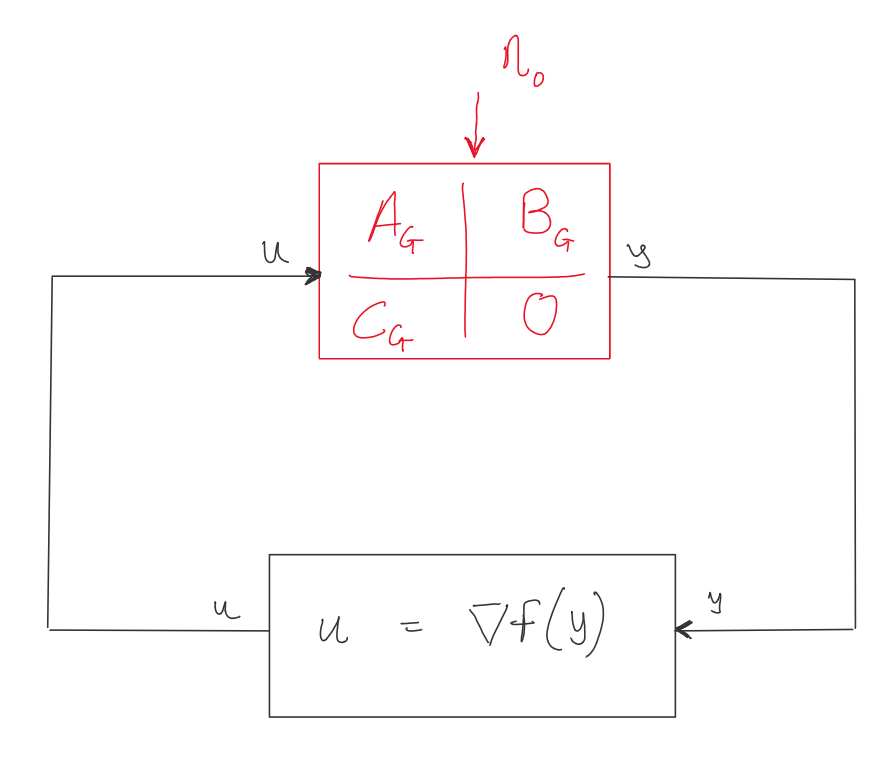
\includegraphics[width=0.8\linewidth,height=0.45\textheight]{figures/loop.PNG}
			\caption{Original loop}
			\label{fig:prob1_6_2}
		\end{minipage}%
		\begin{minipage}{0.5\textwidth}
			\centering
			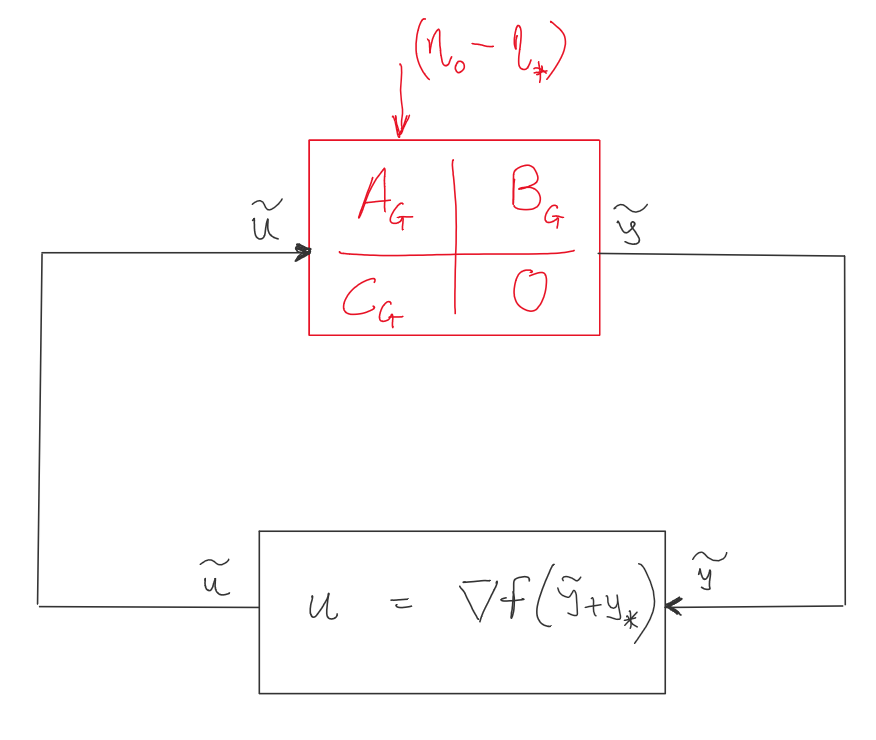
\includegraphics[width=0.8\linewidth,height=0.45\textheight]{figures/loop_dev_vars.PNG}
			\caption{Loop in deviation variables}
			\label{fig:prob1_6_1}
		\end{minipage}
	\end{figure}
\begin{block}{Assumption 1}
	Let $f$ be a differentiable convex field with the minimum at $y_*$ satisfying
	\begin{equation*}
		m||y_1-y_2||^2 \leq  (\nabla f(y_1)-\nabla f(y_2))^T(y_1-y_2) \leq L ||y_1-y_2||^2 \quad \forall y_1,y_2.
	\end{equation*}
	
\end{block}
\end{frame}
%%%%%%%%%%%%%%%%%%%%%%%%%%%%%%%%%%%%%%%%%%%%%%%%%%%%%%%%%%%%%%%%%%%%%
\begin{frame}{Zames Falb IQCs}	
	\begin{figure}[t]
		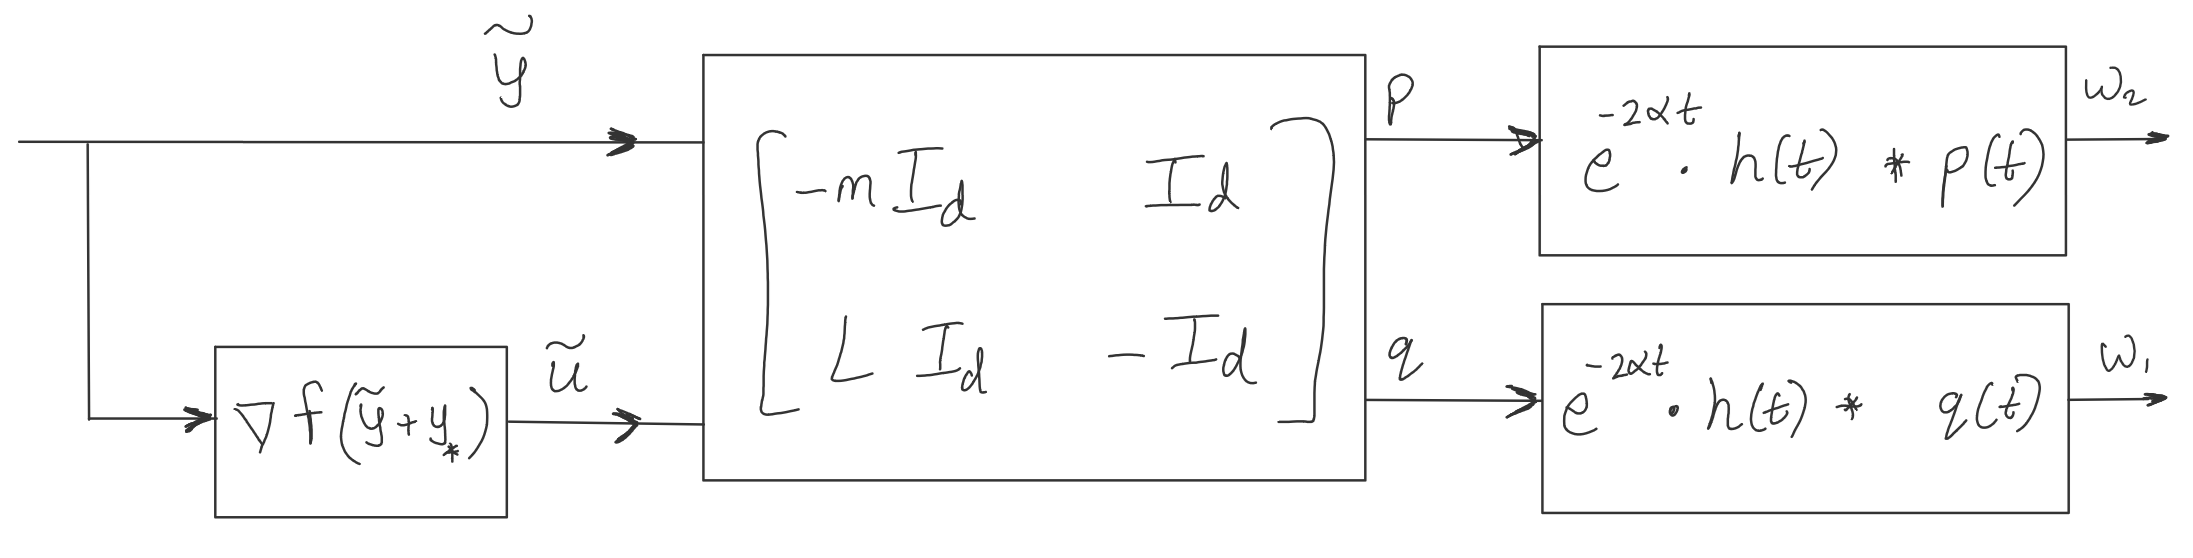
\includegraphics[width=9cm]{figures/signal_definitions_p_q_w.PNG}
		%\input{figures/quadrotor_trajectory}
		%\caption{Block diagram}
		\centering
		%\label{fig:Figure_IQC_paper}
	\end{figure}
\textbf{Theorem:} Let $h \in \mathcal{L}_1(-\infty,\infty)$ satisfy
		\begin{equation} \label{eq:zf_impulse_resp_cond}
			\begin{aligned}
				h(s) &\geq 0, \quad \forall s \in \mathbb{R} \textnormal{ and } \int_{-\infty}^{\infty}h(s)ds &\leq H.
			\end{aligned}
		\end{equation}	
	Then, under the assumptions on $f$, $\forall T \geq 0$ and $\forall \tilde{y} \in \mathcal{L}_{2e}$,	
		\begin{equation}
			\int_0^T e^{2\alpha t}( H p(t)^T q(t) - p(t)^T w_1(t) - q(t)^T w_2(t)) dt \geq 0.
		\end{equation}

\end{frame}
%%%%%%%%%%%%%%%%%%%%%%%%%%%%%%%%%%%%%%%%%%%%%%%%%%%%%%%%%%%%%%%%%%%%%
\begin{frame}{Parameterize $h(t)$}	
	
\begin{itemize}
\item Fix $A_{\nu}=
\begin{bmatrix} 
	\rho   & 0      &\dots     & 0 \\
	1      & \rho   & \ddots        &0  \\
	0      & \ddots      & \ddots     &0  \\
	\vdots & 0      & 1        &\rho  
\end{bmatrix},
B_{\nu}=
\begin{bmatrix} 
	1 \\
	0\\
	\vdots\\
	0 
\end{bmatrix}.$
\item Parameterize $h(t)$ as  
\begin{equation}\label{eq:h_defn}
	\begin{split}
		h(t)&=
		\begin{cases}
			P_1 e^{-A_{\nu}t}B_{\nu}, & \text{if}\ t<0 \\
			P_3 e^{A_{\nu}t}B_{\nu}, & \text{if}\ t\geq 0
		\end{cases}
	\end{split}
\end{equation}
\item If $\textnormal{LMI}(H,P_1,P_3)<0$, conditions on $h(t)$ hold [Scherer, 2013].
\item For searching over only causal(anti-causal) multipleirs, set $P_1=0$ ($P_3=0$)
\item For searching over static multipliers(Circle criterion), set $P_1=0$ and $P_3=0$
\end{itemize}
	
%	\begin{equation}
%		A_{\nu}=
%		\begin{bmatrix} 
%			\rho   & 0      &\dots     & 0 \\
%			1      & \rho   & \ddots        &0  \\
%			0      & \ddots      & \ddots     &0  \\
%			\vdots & 0      & 1        &\rho  
%		\end{bmatrix},
%		B_{\nu}=
%		\begin{bmatrix} 
%			1 \\
%			0\\
%			\vdots\\
%			0 
%		\end{bmatrix}.
%	\end{equation}
	
	
	
\end{frame}
%%%%%%%%%%%%%%%%%%%%%%%%%%%%%%%%%%%%%%%%%%%%%%%%%%%%%%%%%%%%%%%%%%%%%
\begin{frame}{Parameterize $h(t)$}
\begin{figure}[t]
	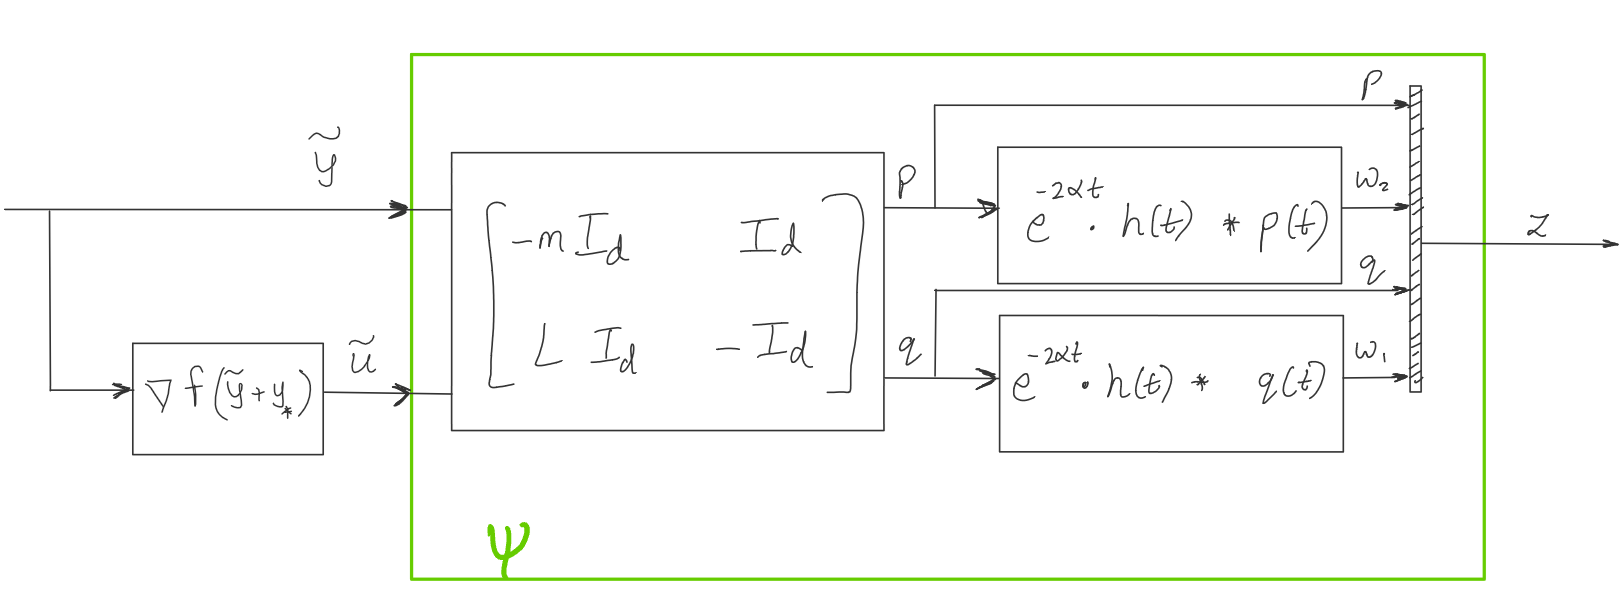
\includegraphics[width=9cm]{figures/signal_definitions.PNG}
	%\input{figures/quadrotor_trajectory}
	%\caption{Block diagram}
	\centering
	%\label{fig:Figure_IQC_paper}
\end{figure}
\begin{equation*}
	( H p^T q - p^T w_1 - q^T w_2)=		
	\tilde{z}^T
	\begin{bmatrix}
		\mathbf{0}  & \begin{bmatrix}
			H  & -P_3 \\
			-P_1^T    & \mathbf{0}
		\end{bmatrix} \\
		*    & \mathbf{0}
	\end{bmatrix}\tilde{z}
\end{equation*}	
Define $\mathbb{P}$ such that every $P \in \mathbb{P}$ generates a valid $h(t)$.	
\begin{equation*}
	\mathbb{P}=\left\{
	\begin{bmatrix}
		\mathbf{0}  & \begin{bmatrix}
			H  & -P_3 \\
			-P_1^T    & \mathbf{0}
		\end{bmatrix} \\
		*    & \mathbf{0}
	\end{bmatrix}: \textnormal{LMI}(H,P_1,P_3)<0
	\right\}
\end{equation*}


%Let the state space realization of $\Psi$ be 
%\begin{equation}\label{eq:ss_Psi}
%	\left[
%	\begin{array}{c|c}
%		A_{\Psi} & B_{\Psi} \\
%		\hline
%		C_{\Psi} & D_{\Psi}
%	\end{array}
%	\right]
%	=
%	\left[
%	\begin{array}{cc|cc}
%		A_{\nu}^{\alpha} \otimes I_d        &\mathbf{0}                         &-B_{\nu}\otimes mI_d       &B_{\nu}\otimes I_d \\
%		\mathbf{0}                          &A_{\nu}^{\alpha} \otimes I_d       &B_{\nu}\otimes LI_d        &-B_{\nu}\otimes I_d \\
%		\hline
%		\mathbf{0}                          &\mathbf{0}                         &-mI_d                      &I_d \\
%		I_{\nu}\otimes I_d                  &\mathbf{0}                         &\mathbf{0}                 &\mathbf{0}\\
%		\mathbf{0}                          &\mathbf{0}                         &LI_d                       &-I_d\\
%		\mathbf{0}                          &I_{\nu}\otimes I_d                 &\mathbf{0}                 &\mathbf{0}
%	\end{array}
%	\right].
%\end{equation}
\end{frame}
%%%%%%%%%%%%%%%%%%%%%%%%%%%%%%%%%%%%%%%%%%%%%%%%%%%%%%%%%%%%%%%%%%%%%
\begin{frame}{Main Results}
\textbf{Theorem:} Under the assumptions on $f$, $\forall T \geq 0$ and $\forall \tilde{y} \in \mathcal{L}_{2e}$,	
	\begin{equation*}
		\int_0^T e^{2\alpha t}\Tilde{z}^T(t) (P \otimes I_d) \Tilde{z}(t) dt \geq 0 \quad \forall P \in \mathbb{P},\forall T \geq 0.
	\end{equation*}
\begin{figure}[t]
	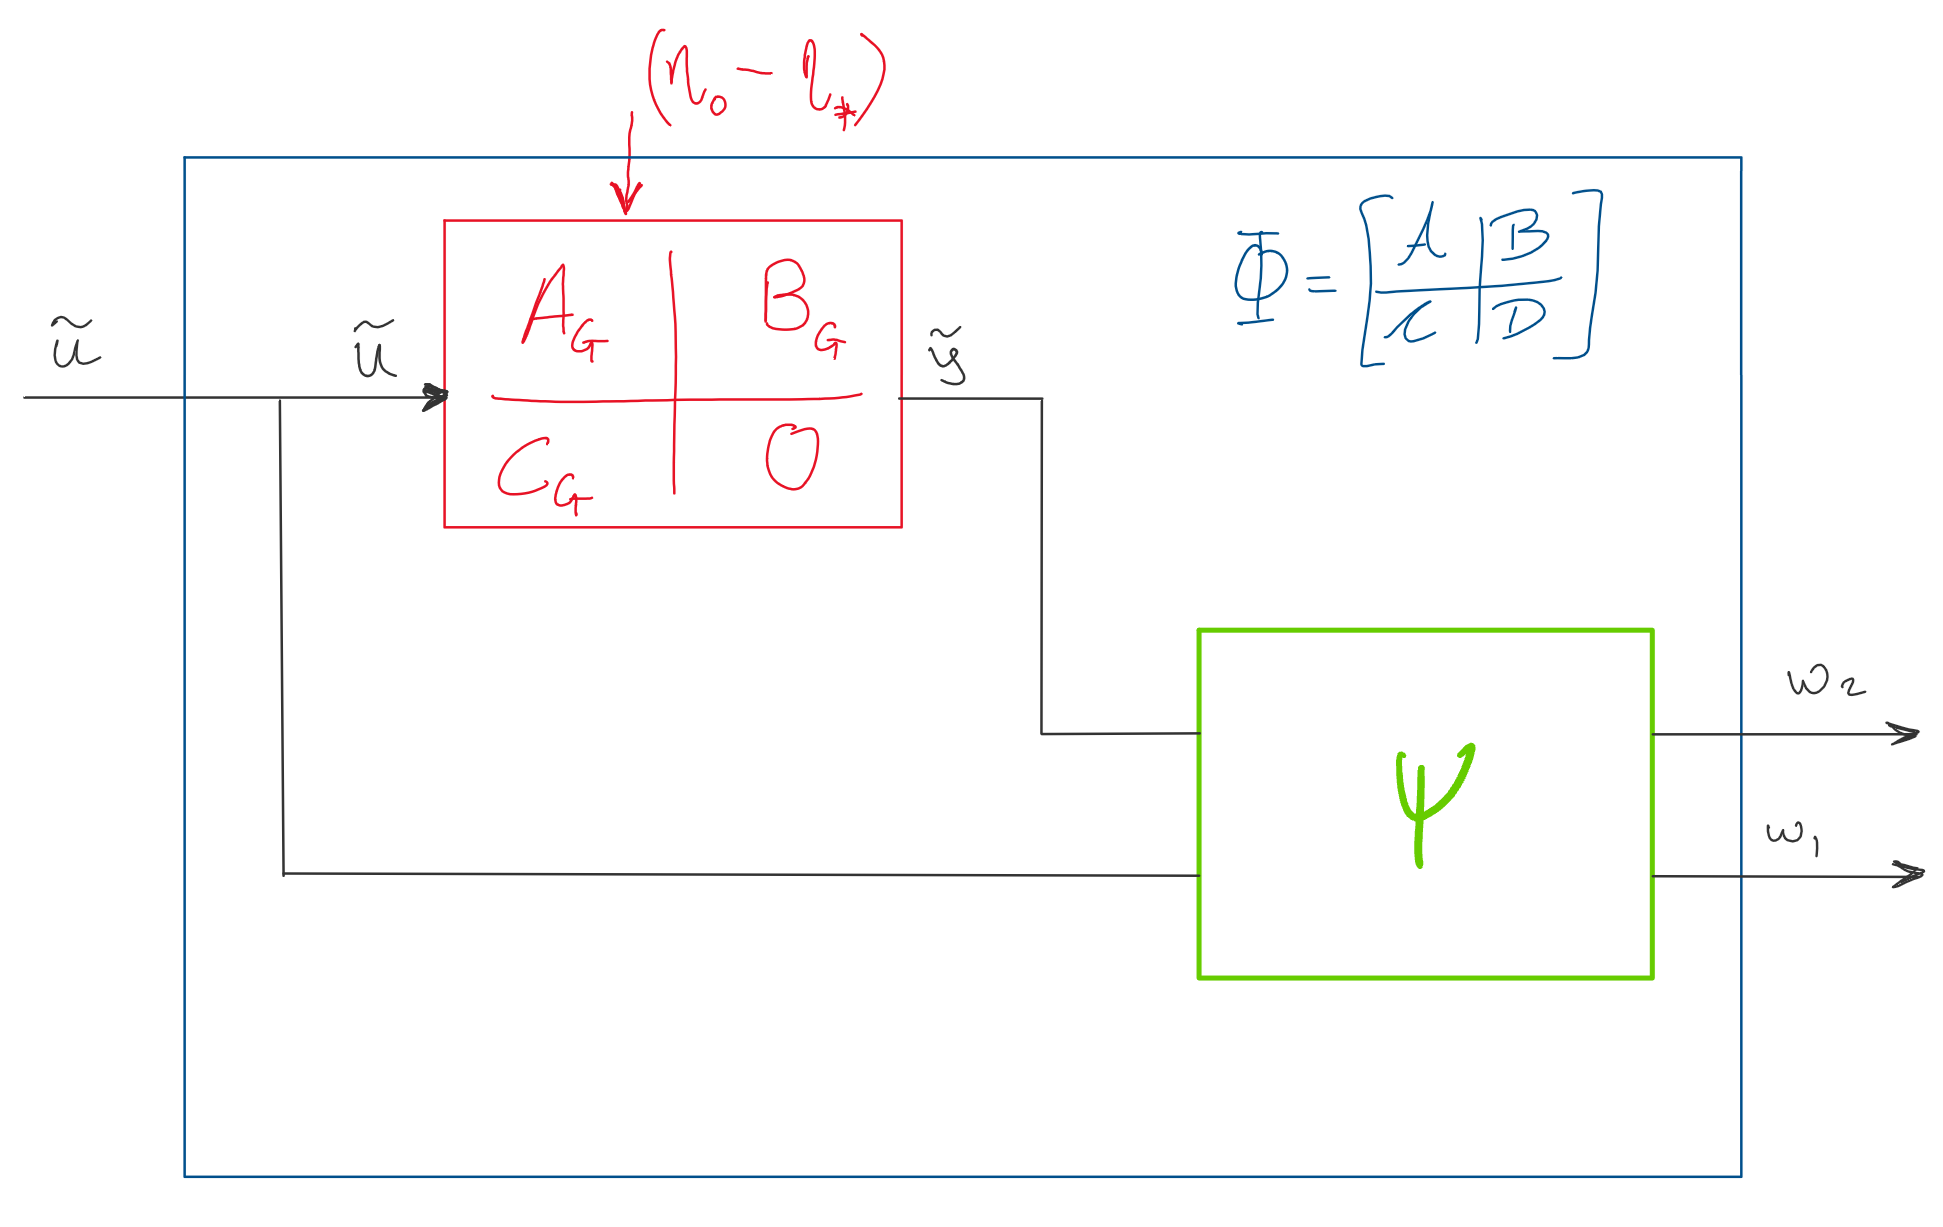
\includegraphics[width=5cm]{figures/Psi_GI.PNG}
	%\input{figures/quadrotor_trajectory}
	% \caption{Block diagram}
	\centering
	%\label{fig:Figure_IQC_paper}
\end{figure}
\textbf{Theorem:} Under the assumptions on $f$, if $\exists \mathcal{X}>0,P \in \mathbb{P}$ such that
\begin{equation*}\label{eq:perf_LMI}
	\begin{bmatrix}
		\mathcal{A}^T\mathcal{X}+\mathcal{X}\mathcal{A}+2\alpha \mathcal{X}  & \mathcal{X}\mathcal{B} \\
		\mathcal{B}^T\mathcal{X}    & \mathbf{0}
	\end{bmatrix}
	+
	\begin{bmatrix}
		\mathcal{C}^T \\
		\mathcal{D}^T 
	\end{bmatrix}
	( P\otimes I_d)
	\begin{bmatrix}
		\mathcal{C} & \mathcal{D} 
	\end{bmatrix}
	\leq 
	0,
\end{equation*}
then, $||\Tilde{y}(t)||\leq \kappa e^{-\alpha t}$ holds for all $t\geq 0$, 
\end{frame}
%%%%%%%%%%%%%%%%%%%%%%%%%%%%%%%%%%%%%%%%%%%%%%%%%%%%%%%%%%%%%%%%%%%%%
%\begin{frame}{Theory}
%	\begin{figure}[t]
%	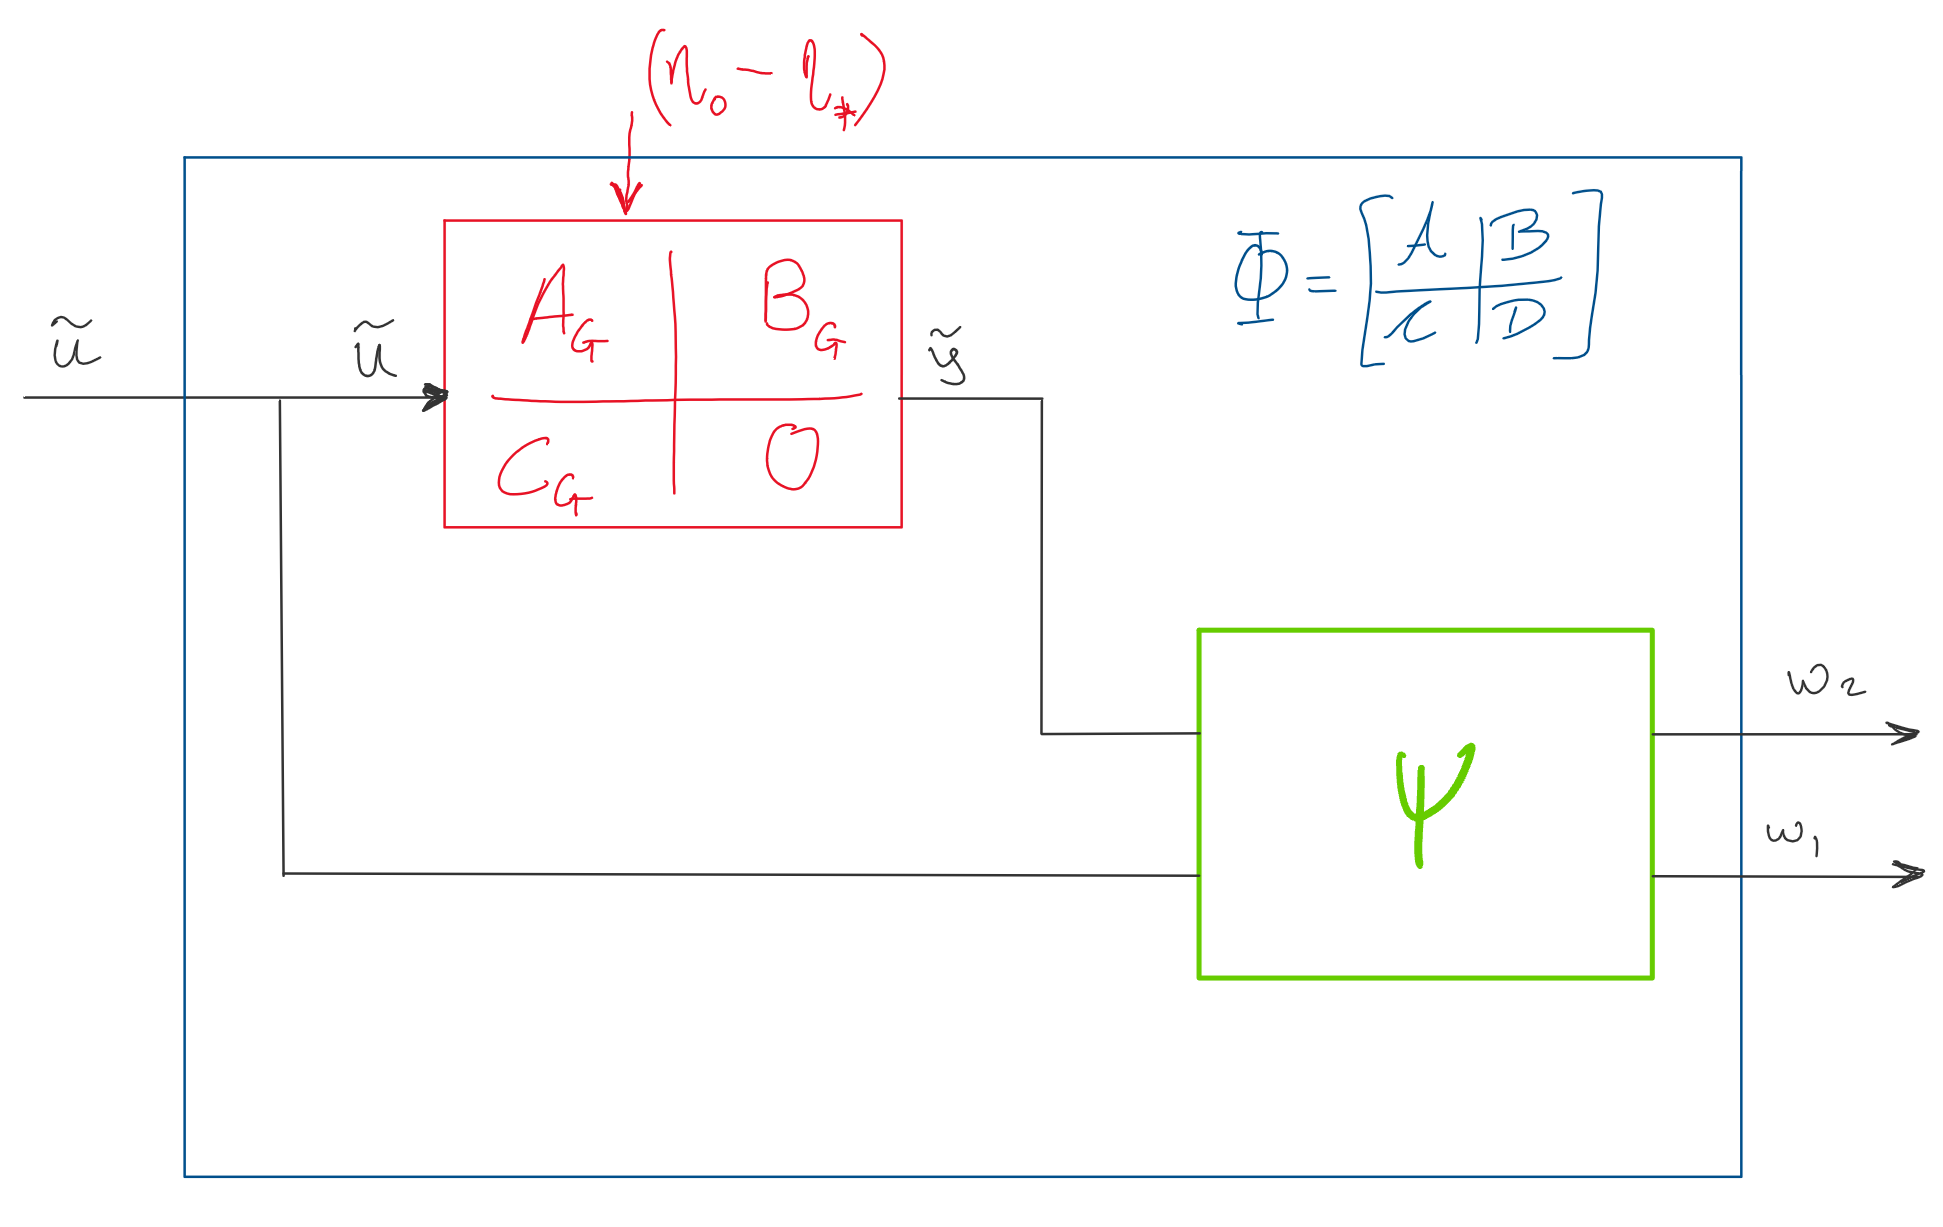
\includegraphics[width=5cm]{figures/Psi_GI.PNG}
%	%\input{figures/quadrotor_trajectory}
%	% \caption{Block diagram}
%	\centering
%	%\label{fig:Figure_IQC_paper}
%	\end{figure}
%\begin{theorem}\label{theom:theorem_perf_analysis}
%	If $\exists \mathcal{X}>0,P \in \mathbb{P}$ such that
%	\begin{equation}\label{eq:perf_LMI}
%		\begin{bmatrix}
%			\mathcal{A}^T\mathcal{X}+\mathcal{X}\mathcal{A}+2\alpha \mathcal{X}  & \mathcal{X}\mathcal{B} \\
%			\mathcal{B}^T\mathcal{X}    & \mathbf{0}
%		\end{bmatrix}
%		+
%		\begin{bmatrix}
%			\mathcal{C}^T \\
%			\mathcal{D}^T 
%		\end{bmatrix}
%		( P\otimes I_d)
%		\begin{bmatrix}
%			\mathcal{C} & \mathcal{D} 
%		\end{bmatrix}
%		\leq 
%		0,
%	\end{equation}
%	then, $y$ converges exponentially to $y_*$ with rate $\alpha$, i.e., $\exists \kappa \geq 0$ such that  
%	$||\Tilde{y}(t)||\leq \kappa e^{-\alpha t}$ holds for all $t\geq 0$.
%\end{theorem}
%\end{frame}
%%%%%%%%%%%%%%%%%%%%%%%%%%%%%%%%%%%%%%%%%%%%%%%%%%%%%%%%%%%%%%%%%%%%%
\begin{frame}{Numerical results: Quadrotor}
	\begin{figure}[!htb]
			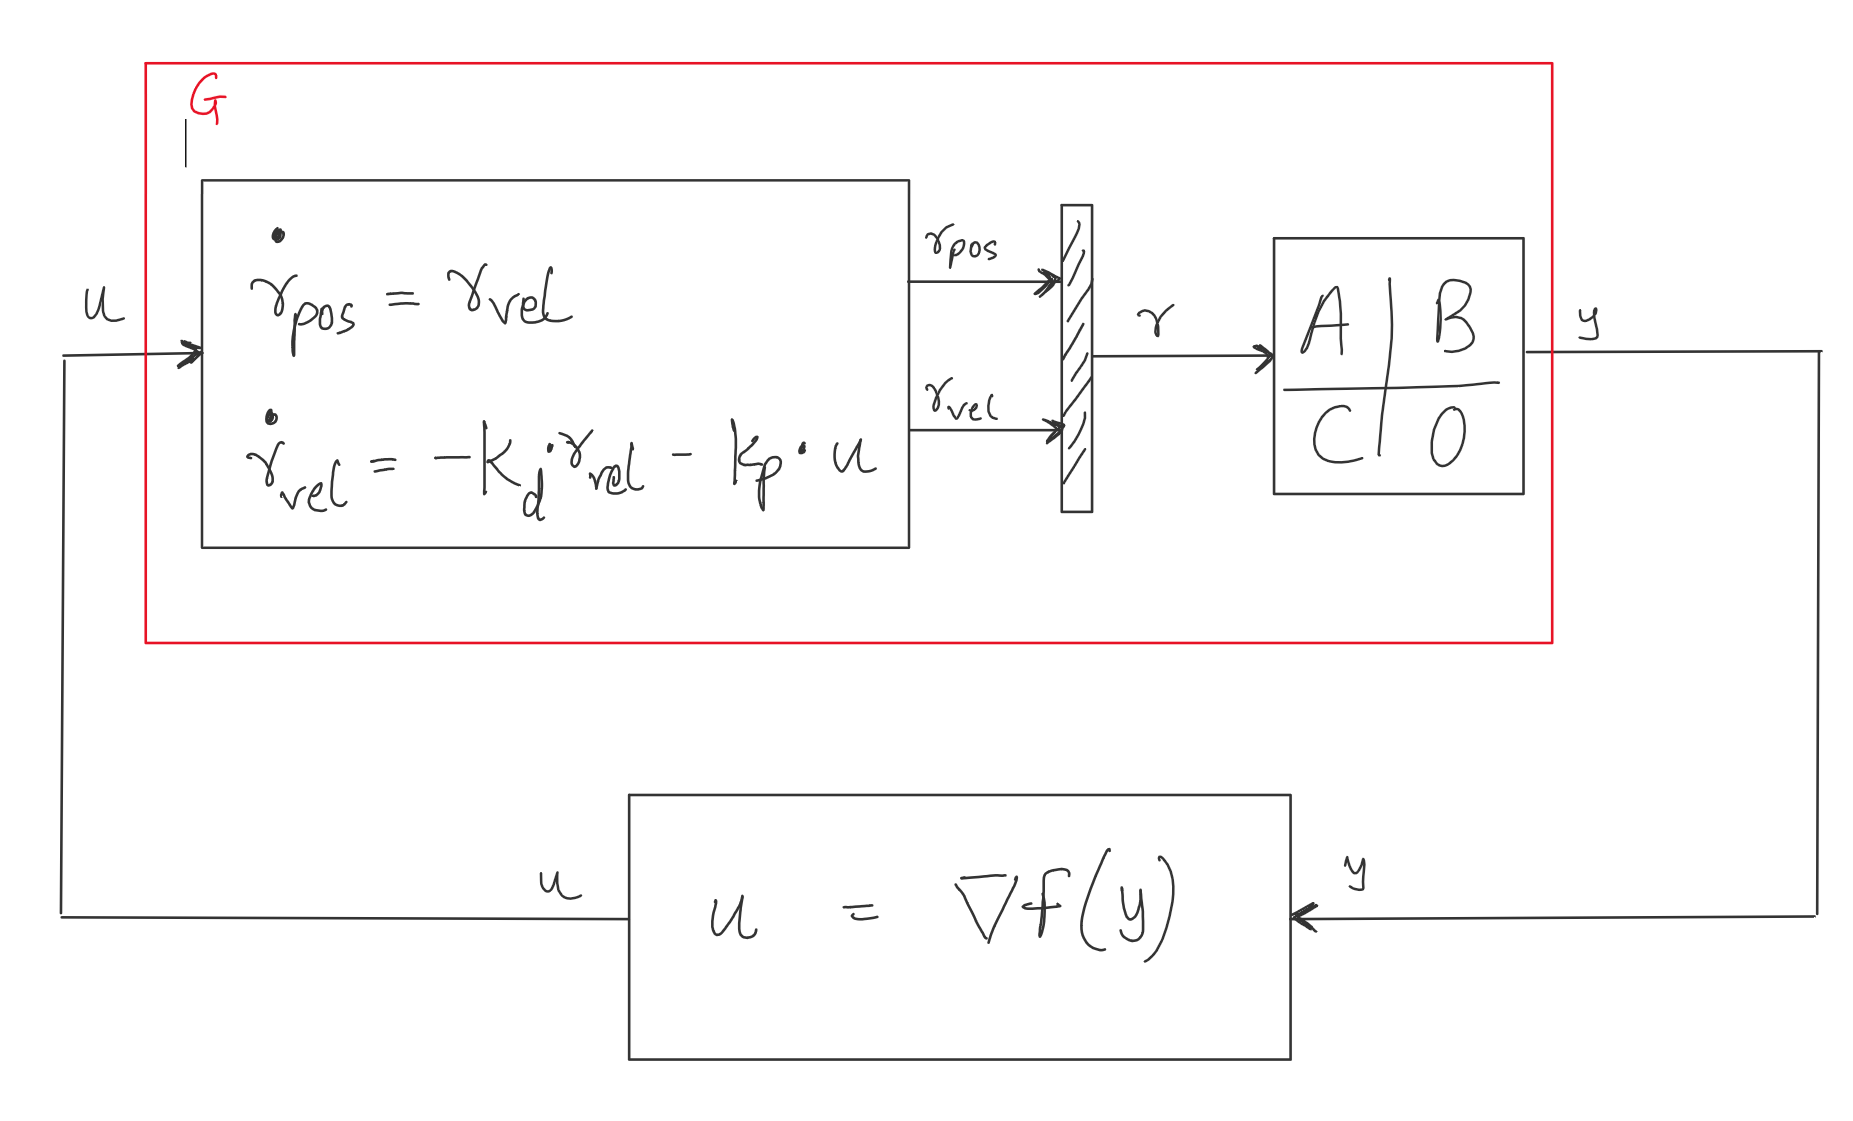
\includegraphics[width=6cm]{figures/Figure_IQC_paper.PNG}		
			\centering	
	\end{figure}
	\begin{block}{Setup}
		\begin{itemize}
			\item Linearized quadrotor model + LQR local controller
			\item Questions:
				  \begin{itemize}
				  	\item How robust is the given controller for different fields?
				  	\item How do we select the PD gains for the pre-filter?
				  	\item How conservative are the estimates on the rates of convergence?
			  	  \end{itemize}
		\end{itemize}
	\end{block}	
\end{frame}
%%%%%%%%%%%%%%%%%%%%%%%%%%%%%%%%%%%%%%%%%%%%%%%%%%%%%%%%%%%%%%%%%%%%%
\begin{frame}{Numerical results: Robustness with respect to field}	
	\begin{figure}[t]
		%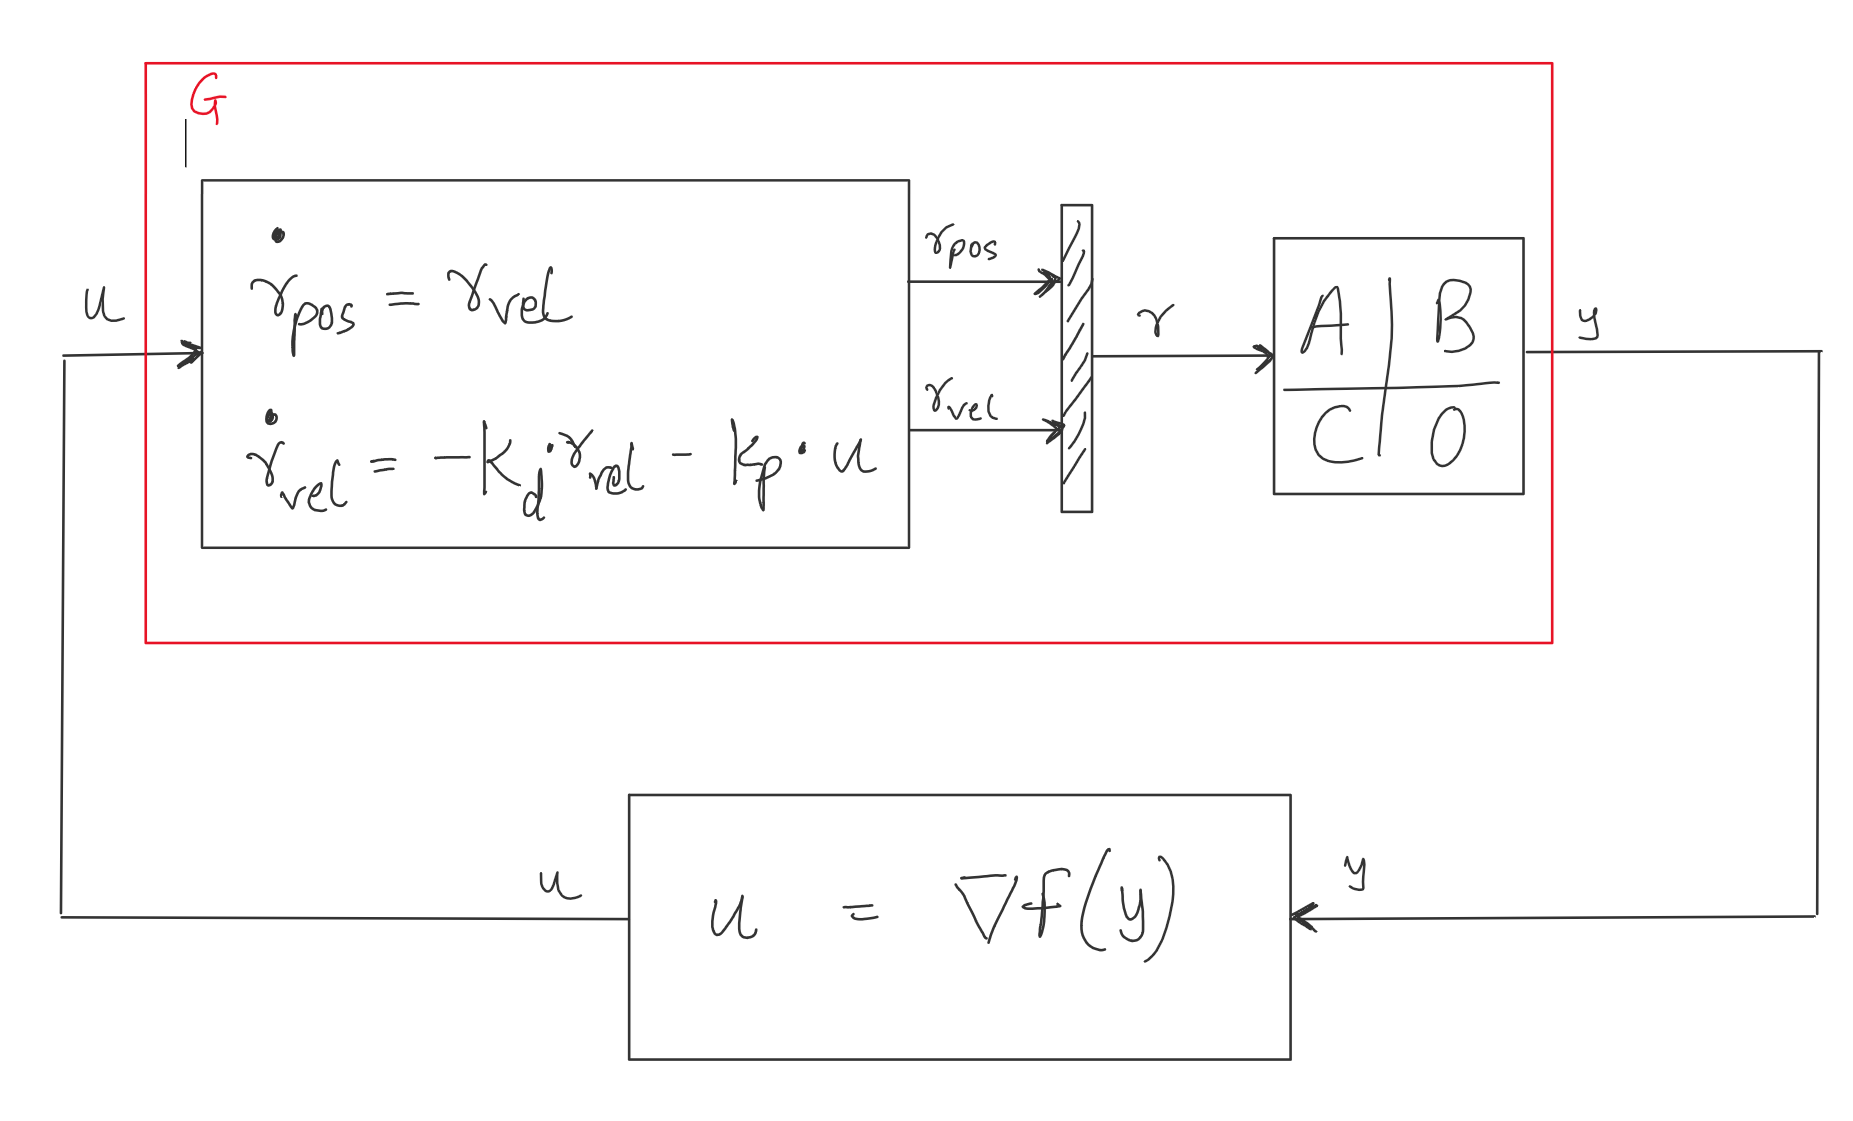
\includegraphics[width=8cm]{figures/Figure_IQC_paper.PNG}
		% This file was created by matlab2tikz.
%
%The latest updates can be retrieved from
%  http://www.mathworks.com/matlabcentral/fileexchange/22022-matlab2tikz-matlab2tikz
%where you can also make suggestions and rate matlab2tikz.
%
\definecolor{mycolor1}{rgb}{0.00000,1.00000,1.00000}%
%
\begin{tikzpicture}

\begin{axis}[%
width=2.321in,
height=2.266in,
at={(1in,2in)},
scale only axis,
xmin=1,
xmax=9,
xlabel style={font=\color{white!15!black}},
xlabel={$L$},
ymin=0,
ymax=0.5,
ylabel style={font=\color{white!15!black}},
ylabel={$\alpha$},
axis background/.style={fill=white},
title style={font=\bfseries},
title={},
legend style={legend cell align=left, align=left, draw=white!15!black}
]
\addplot [color=red]
  table[row sep=crcr]{%
1	0.4119873046875\\
1.1	0.3741455078125\\
1.2	0.3472900390625\\
1.3	0.325927734375\\
1.4	0.3076171875\\
1.5	0.291748046875\\
1.6	0.277099609375\\
1.7	0.263671875\\
1.8	0.2508544921875\\
1.9	0.2386474609375\\
2	0.2276611328125\\
2.1	0.2166748046875\\
2.2	0.2069091796875\\
2.3	0.1971435546875\\
2.4	0.1873779296875\\
2.5	0.17822265625\\
2.6	0.1690673828125\\
2.7	0.1605224609375\\
2.8	0.152587890625\\
2.9	0.14404296875\\
3	0.1361083984375\\
3.1	0.1287841796875\\
3.2	0.120849609375\\
3.3	0.113525390625\\
3.4	0.106201171875\\
3.5	0.0994873046875\\
3.6	0.0921630859375\\
3.7	0.08544921875\\
3.8	0.0787353515625\\
3.9	0.072021484375\\
4	0.06591796875\\
4.1	0.0592041015625\\
4.2	0.0531005859375\\
4.3	0.0469970703125\\
4.4	0.0408935546875\\
4.5	0.0347900390625\\
4.6	0.029296875\\
4.7	0.023193359375\\
4.8	0.0177001953125\\
4.9	0.01220703125\\
5	0.006103515625\\
5.1	0.0006103515625\\
5.2	-1\\
5.3	-1\\
5.4	-1\\
5.5	-1\\
5.6	-1\\
5.7	-1\\
5.8	-1\\
5.9	-1\\
6	-1\\
6.1	-1\\
6.2	-1\\
6.3	-1\\
6.4	-1\\
6.5	-1\\
6.6	-1\\
6.7	-1\\
6.8	-1\\
6.9	-1\\
7	-1\\
7.1	-1\\
7.2	-1\\
7.3	-1\\
7.4	-1\\
7.5	-1\\
7.6	-1\\
7.7	-1\\
7.8	-1\\
7.9	-1\\
8	-1\\
8.1	-1\\
8.2	-1\\
8.3	-1\\
8.4	-1\\
8.5	-1\\
8.6	-1\\
8.7	-1\\
8.8	-1\\
8.9	-1\\
9	-1\\
9.1	-1\\
9.2	-1\\
9.3	-1\\
9.4	-1\\
9.5	-1\\
9.6	-1\\
9.7	-1\\
9.8	-1\\
9.9	-1\\
10	-1\\
};
\addlegendentry{CC}

\addplot [color=green]
  table[row sep=crcr]{%
1	0.4119873046875\\
1.1	0.38330078125\\
1.2	0.3643798828125\\
1.3	0.350341796875\\
1.4	0.33935546875\\
1.5	0.32958984375\\
1.6	0.321044921875\\
1.7	0.313720703125\\
1.8	0.306396484375\\
1.9	0.30029296875\\
2	0.2935791015625\\
2.1	0.2880859375\\
2.2	0.281982421875\\
2.3	0.2764892578125\\
2.4	0.27099609375\\
2.5	0.2655029296875\\
2.6	0.260009765625\\
2.7	0.2545166015625\\
2.8	0.2490234375\\
2.9	0.2435302734375\\
3	0.2386474609375\\
3.1	0.233154296875\\
3.2	0.2276611328125\\
3.3	0.2227783203125\\
3.4	0.21728515625\\
3.5	0.2117919921875\\
3.6	0.2069091796875\\
3.7	0.201416015625\\
3.8	0.196533203125\\
3.9	0.1910400390625\\
4	0.1861572265625\\
4.1	0.1806640625\\
4.2	0.17578125\\
4.3	0.1708984375\\
4.4	0.1654052734375\\
4.5	0.1605224609375\\
4.6	0.1556396484375\\
4.7	0.150146484375\\
4.8	0.145263671875\\
4.9	0.140380859375\\
5	0.135498046875\\
5.1	0.130615234375\\
5.2	0.125732421875\\
5.3	0.120849609375\\
5.4	0.115966796875\\
5.5	0.111083984375\\
5.6	0.1068115234375\\
5.7	0.1019287109375\\
5.8	0.0970458984375\\
5.9	0.0927734375\\
6	0.087890625\\
6.1	0.0836181640625\\
6.2	0.0787353515625\\
6.3	0.074462890625\\
6.4	0.069580078125\\
6.5	0.0653076171875\\
6.6	0.06103515625\\
6.7	0.05615234375\\
6.8	0.0518798828125\\
6.9	0.047607421875\\
7	0.0433349609375\\
7.1	0.0390625\\
7.2	0.0347900390625\\
7.3	0.030517578125\\
7.4	0.0262451171875\\
7.5	0.02197265625\\
7.6	0.0177001953125\\
7.7	0.0140380859375\\
7.8	0.009765625\\
7.9	0.0054931640625\\
8	0.0018310546875\\
8.1	-1\\
8.2	-1\\
8.3	-1\\
8.4	-1\\
8.5	-1\\
8.6	-1\\
8.7	-1\\
8.8	-1\\
8.9	-1\\
9	-1\\
9.1	-1\\
9.2	-1\\
9.3	-1\\
9.4	-1\\
9.5	-1\\
9.6	-1\\
9.7	-1\\
9.8	-1\\
9.9	-1\\
10	-1\\
};
\addlegendentry{ZFb causal}

\addplot [color=blue, only marks, mark=o, mark options={solid, blue}]
  table[row sep=crcr]{%
1	0.4119873046875\\
1.1	0.3741455078125\\
1.2	0.3472900390625\\
1.3	0.325927734375\\
1.4	0.3076171875\\
1.5	0.291748046875\\
1.6	0.277099609375\\
1.7	0.263671875\\
1.8	0.2508544921875\\
1.9	0.2386474609375\\
2	0.2276611328125\\
2.1	0.2166748046875\\
2.2	0.2069091796875\\
2.3	0.1971435546875\\
2.4	0.1873779296875\\
2.5	0.17822265625\\
2.6	0.1690673828125\\
2.7	0.1605224609375\\
2.8	0.152587890625\\
2.9	0.14404296875\\
3	0.1361083984375\\
3.1	0.1287841796875\\
3.2	0.120849609375\\
3.3	0.113525390625\\
3.4	0.106201171875\\
3.5	0.0994873046875\\
3.6	0.0921630859375\\
3.7	0.08544921875\\
3.8	0.0787353515625\\
3.9	0.072021484375\\
4	0.06591796875\\
4.1	0.0592041015625\\
4.2	0.0531005859375\\
4.3	0.0469970703125\\
4.4	0.0408935546875\\
4.5	0.0347900390625\\
4.6	0.029296875\\
4.7	0.023193359375\\
4.8	0.0177001953125\\
4.9	0.01220703125\\
5	0.006103515625\\
5.1	0.0006103515625\\
5.2	-1\\
5.3	-1\\
5.4	-1\\
5.5	-1\\
5.6	-1\\
5.7	-1\\
5.8	-1\\
5.9	-1\\
6	-1\\
6.1	-1\\
6.2	-1\\
6.3	-1\\
6.4	-1\\
6.5	-1\\
6.6	-1\\
6.7	-1\\
6.8	-1\\
6.9	-1\\
7	-1\\
7.1	-1\\
7.2	-1\\
7.3	-1\\
7.4	-1\\
7.5	-1\\
7.6	-1\\
7.7	-1\\
7.8	-1\\
7.9	-1\\
8	-1\\
8.1	-1\\
8.2	-1\\
8.3	-1\\
8.4	-1\\
8.5	-1\\
8.6	-1\\
8.7	-1\\
8.8	-1\\
8.9	-1\\
9	-1\\
9.1	-1\\
9.2	-1\\
9.3	-1\\
9.4	-1\\
9.5	-1\\
9.6	-1\\
9.7	-1\\
9.8	-1\\
9.9	-1\\
10	-1\\
};
\addlegendentry{ZFb anti causal}

\addplot [color=mycolor1]
  table[row sep=crcr]{%
1	0.4119873046875\\
1.1	0.404052734375\\
1.2	0.3955078125\\
1.3	0.3875732421875\\
1.4	0.379638671875\\
1.5	0.3717041015625\\
1.6	0.3643798828125\\
1.7	0.3564453125\\
1.8	0.34912109375\\
1.9	0.3411865234375\\
2	0.3338623046875\\
2.1	0.3265380859375\\
2.2	0.3192138671875\\
2.3	0.3125\\
2.4	0.30517578125\\
2.5	0.2984619140625\\
2.6	0.2911376953125\\
2.7	0.284423828125\\
2.8	0.2777099609375\\
2.9	0.27099609375\\
3	0.2642822265625\\
3.1	0.2581787109375\\
3.2	0.25146484375\\
3.3	0.245361328125\\
3.4	0.2386474609375\\
3.5	0.2325439453125\\
3.6	0.2264404296875\\
3.7	0.2203369140625\\
3.8	0.2142333984375\\
3.9	0.2081298828125\\
4	0.20263671875\\
4.1	0.196533203125\\
4.2	0.1910400390625\\
4.3	0.1849365234375\\
4.4	0.179443359375\\
4.5	0.1739501953125\\
4.6	0.16845703125\\
4.7	0.1629638671875\\
4.8	0.157470703125\\
4.9	0.1519775390625\\
5	0.146484375\\
5.1	0.1409912109375\\
5.2	0.1361083984375\\
5.3	0.130615234375\\
5.4	0.125732421875\\
5.5	0.1202392578125\\
5.6	0.1153564453125\\
5.7	0.1104736328125\\
5.8	0.1055908203125\\
5.9	0.1007080078125\\
6	0.0958251953125\\
6.1	0.0909423828125\\
6.2	0.0860595703125\\
6.3	0.0811767578125\\
6.4	0.0762939453125\\
6.5	0.072021484375\\
6.6	0.067138671875\\
6.7	0.062255859375\\
6.8	0.0579833984375\\
6.9	0.0537109375\\
7	0.048828125\\
7.1	0.0445556640625\\
7.2	0.040283203125\\
7.3	0.035400390625\\
7.4	0.0311279296875\\
7.5	0.02685546875\\
7.6	0.0225830078125\\
7.7	0.018310546875\\
7.8	0.0140380859375\\
7.9	0.0103759765625\\
8	0.006103515625\\
8.1	0.0018310546875\\
8.2	-1\\
8.3	-1\\
8.4	-1\\
8.5	-1\\
8.6	-1\\
8.7	-1\\
8.8	-1\\
8.9	-1\\
9	-1\\
9.1	-1\\
9.2	-1\\
9.3	-1\\
9.4	-1\\
9.5	-1\\
9.6	-1\\
9.7	-1\\
9.8	-1\\
9.9	-1\\
10	-1\\
};
\addlegendentry{ZFb non causal}

\addplot [color=black, only marks, mark=o, mark options={solid, black}]
  table[row sep=crcr]{%
1	0.412331651029502\\
1.1	0.404104631075646\\
1.2	0.395974289263065\\
1.3	0.387939741864961\\
1.4	0.380000019452198\\
1.5	0.372154077971261\\
1.6	0.364400808966183\\
1.7	0.356739048974318\\
1.8	0.349167588131177\\
1.9	0.341685178023271\\
2	0.334290538830462\\
2.1	0.326982365800579\\
2.2	0.319759335099553\\
2.3	0.312620109080054\\
2.4	0.305563341010739\\
2.5	0.298587679307016\\
2.6	0.291691771302537\\
2.7	0.284874266598906\\
2.8	0.278133820029051\\
2.9	0.271469094267668\\
3	0.26487876212005\\
3.1	0.258361508518492\\
3.2	0.251916032253452\\
3.3	0.245541047464569\\
3.4	0.239235284914789\\
3.5	0.232997493068939\\
3.6	0.226826438996406\\
3.7	0.220720909115899\\
3.8	0.214679709798701\\
3.9	0.208701667845465\\
4	0.202785630850187\\
4.1	0.196930467463774\\
4.2	0.191135067568535\\
4.3	0.185398342373745\\
4.4	0.179719224441609\\
4.5	0.174096667651941\\
4.6	0.168529647113125\\
4.7	0.163017159026185\\
4.8	0.157558220508055\\
4.9	0.152151869379587\\
5	0.146797163923227\\
5.1	0.141493182614812\\
5.2	0.136239023833451\\
5.3	0.131033805553032\\
5.4	0.125876665018558\\
5.5	0.120766758410098\\
5.6	0.115703260496917\\
5.7	0.110685364283959\\
5.8	0.105712280652736\\
5.9	0.100783237998324\\
6	0.0958974818640143\\
6.1	0.091054274575032\\
6.2	0.0862528948724395\\
6.3	0.0814926375483512\\
6.4	0.0767728130832954\\
6.5	0.072092747286594\\
6.6	0.0674517809403497\\
6.7	0.062849269447712\\
6.8	0.0582845824858739\\
6.9	0.0537571036642326\\
7	0.0492662301880663\\
7.1	0.0448113725280309\\
7.2	0.0403919540956924\\
7.3	0.0360074109253169\\
7.4	0.0316571913620152\\
7.5	0.0273407557564156\\
7.6	0.0230575761658652\\
7.7	0.0188071360622775\\
7.8	0.0145889300465936\\
7.9	0.0104024635698768\\
8	0.00624725266099616\\
8.1	0.00212282366089683\\
8.2	-0.00197128703662988\\
8.3	-0.00603553323776879\\
8.4	-0.0100703591950907\\
8.5	-0.0140761998477345\\
8.6	-0.0180534810554153\\
8.7	-0.0220026198263578\\
8.8	-0.0259240245392573\\
8.9	-0.0298180951594347\\
9	-0.0336852234492339\\
9.1	-0.0375257931728344\\
9.2	-0.0413401802955638\\
9.3	-0.0451287531778723\\
9.4	-0.0488918727640491\\
9.5	-0.0526298927658563\\
9.6	-0.0563431598411483\\
9.7	-0.0600320137676526\\
9.8	-0.0636967876120013\\
9.9	-0.0673378078941474\\
10	-0.0709553947472893\\
};
\addlegendentry{Example field}

\end{axis}

\begin{axis}[%
width=5.833in,
height=4.375in,
at={(0in,0in)},
scale only axis,
xmin=0,
xmax=1,
ymin=0,
ymax=1,
axis line style={draw=none},
ticks=none,
axis x line*=bottom,
axis y line*=left
]
\end{axis}
\end{tikzpicture}%
		\caption{Robustness for Quadrotor and $m=1$}
		\centering
		\label{fig:quadrotor_robustness}
	\end{figure}
\end{frame}
%%%%%%%%%%%%%%%%%%%%%%%%%%%%%%%%%%%%%%%%%%%%%%%%%%%%%%%%%%%%%%%%%%%%%
\begin{frame}{Numerical results: Performance curves for kp,kd}
	\begin{figure}[t]
		%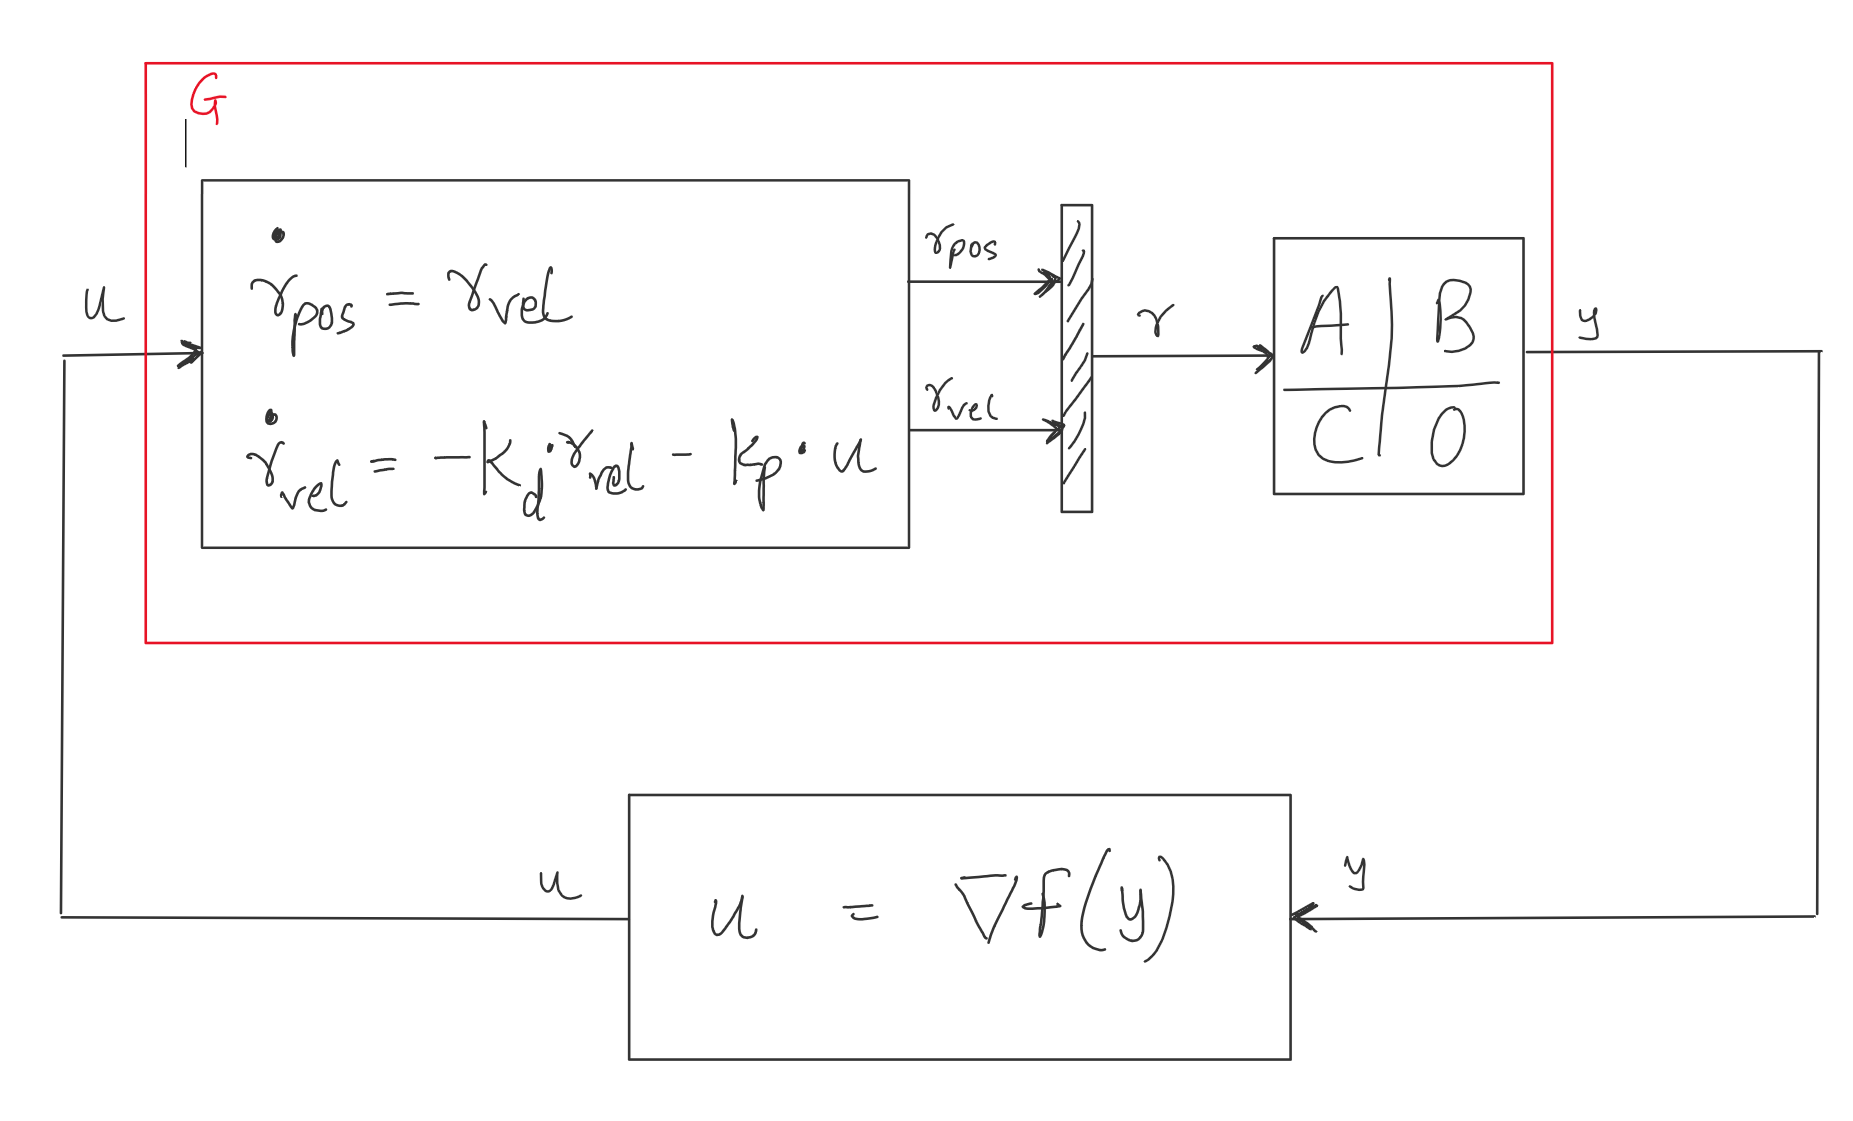
\includegraphics[width=8cm]{figures/Figure_IQC_paper.PNG}
		% This file was created by matlab2tikz.
%
%The latest updates can be retrieved from
%  http://www.mathworks.com/matlabcentral/fileexchange/22022-matlab2tikz-matlab2tikz
%where you can also make suggestions and rate matlab2tikz.
%
\definecolor{mycolor1}{rgb}{0.00000,0.44700,0.74100}%
\definecolor{mycolor2}{rgb}{0.85000,0.32500,0.09800}%
%
\begin{tikzpicture}

\begin{axis}[%
width=2.321in,
height=2.266in,
at={(1in,2in)},
scale only axis,
xmin=5,
xmax=20,
xlabel style={font=\color{white!15!black}},
xlabel={$\frac{k_d}{k_p}$},
ymin=0,
ymax=0.2,
ylabel style={font=\color{white!15!black}},
ylabel={$\alpha$},
axis background/.style={fill=white},
title style={font=\bfseries},
title={},
legend style={legend cell align=left, align=left, draw=white!15!black}
]
\addplot [color=mycolor1, only marks, mark=asterisk, mark options={solid, mycolor1}]
  table[row sep=crcr]{%
0.2	-1\\
0.6	-1\\
1	-1\\
1.4	-1\\
1.8	-1\\
2.2	-1\\
2.6	-1\\
3	-1\\
3.4	-1\\
3.8	-1\\
4.2	-1\\
4.6	-1\\
5	-1\\
5.4	-1\\
5.8	-1\\
6.2	-1\\
6.6	-1\\
7	-1\\
7.4	-1\\
7.8	-1\\
8.2	-1\\
8.6	-1\\
9	-1\\
9.4	-1\\
9.8	-1\\
10.2	0.001220703125\\
10.6	0.008544921875\\
11	0.0152587890625\\
11.4	0.0213623046875\\
11.8	0.0262451171875\\
12.2	0.03173828125\\
12.6	0.0360107421875\\
13	0.040283203125\\
13.4	0.0439453125\\
13.8	0.0469970703125\\
14.2	0.050048828125\\
14.6	0.052490234375\\
15	0.054931640625\\
15.4	0.0567626953125\\
15.8	0.0579833984375\\
16.2	0.0592041015625\\
16.6	0.059814453125\\
17	0.0604248046875\\
17.4	0.0604248046875\\
17.8	0.0604248046875\\
18.2	0.059814453125\\
18.6	0.05859375\\
19	0.057373046875\\
19.4	0.05615234375\\
19.8	0.054931640625\\
};
\addlegendentry{CC}

\addplot [color=mycolor2, only marks, mark=asterisk, mark options={solid, mycolor2}]
  table[row sep=crcr]{%
0.2	-1\\
0.6	-1\\
1	-1\\
1.4	-1\\
1.8	-1\\
2.2	-1\\
2.6	-1\\
3	-1\\
3.4	-1\\
3.8	-1\\
4.2	-1\\
4.6	-1\\
5	-1\\
5.4	0.0164794921875\\
5.8	0.0408935546875\\
6.2	0.0628662109375\\
6.6	0.0830078125\\
7	0.101318359375\\
7.4	0.118408203125\\
7.8	0.13427734375\\
8.2	0.1483154296875\\
8.6	0.147705078125\\
9	0.13916015625\\
9.4	0.1312255859375\\
9.8	0.12451171875\\
10.2	0.118408203125\\
10.6	0.1129150390625\\
11	0.1080322265625\\
11.4	0.1031494140625\\
11.8	0.098876953125\\
12.2	0.09521484375\\
12.6	0.091552734375\\
13	0.0885009765625\\
13.4	0.08544921875\\
13.8	0.0823974609375\\
14.2	0.079345703125\\
14.6	0.076904296875\\
15	0.074462890625\\
15.4	0.0726318359375\\
15.8	0.0701904296875\\
16.2	0.068359375\\
16.6	0.0665283203125\\
17	0.064697265625\\
17.4	0.0634765625\\
17.8	0.0616455078125\\
18.2	0.059814453125\\
18.6	0.05859375\\
19	0.057373046875\\
19.4	0.05615234375\\
19.8	0.054931640625\\
};
\addlegendentry{ZFb}

\end{axis}

\begin{axis}[%
width=5.833in,
height=4.375in,
at={(0in,0in)},
scale only axis,
xmin=0,
xmax=1,
ymin=0,
ymax=1,
axis line style={draw=none},
ticks=none,
axis x line*=bottom,
axis y line*=left
]
\end{axis}
\end{tikzpicture}%
		\caption{Robustness for Quadrotor and $m=1$}
		\centering
		\label{fig:optimal_kd_kp_ratio}
	\end{figure}
\end{frame}
%%%%%%%%%%%%%%%%%%%%%%%%%%%%%%%%%%%%%%%%%%%%%%%%%%%%%%%%%%%%%%%%%%%%%
\begin{frame}{Numerical results: Quadrotor Trajectory}	
	\begin{figure}[t]
		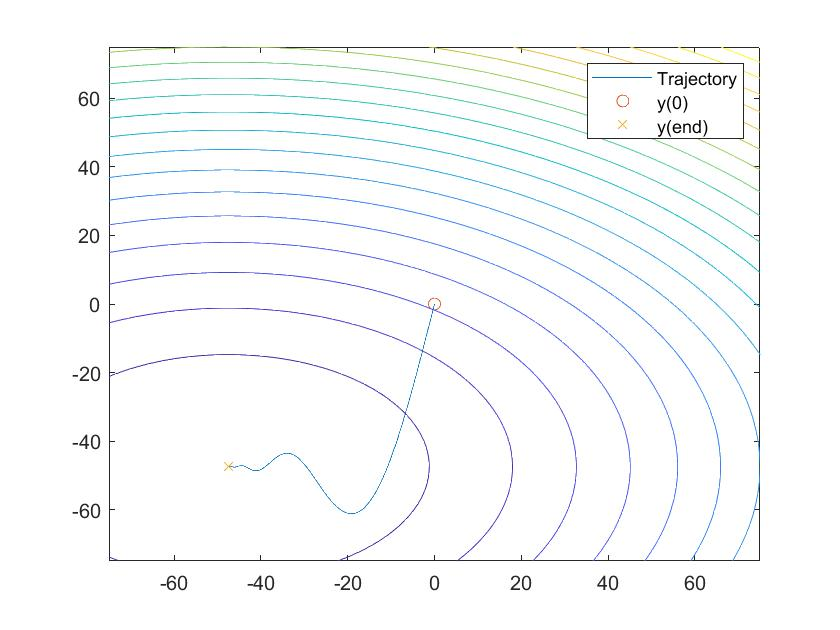
\includegraphics[width=8cm]{figures/quadrotor_trajectory.JPG}
		%\input{figures/quadrotor_trajectory}
		\caption{Robustness for Quadrotor and $m=1$}
		\centering
		\label{fig:quadrotor_trajectory}
	\end{figure}
\end{frame}

%%%%%%%%%%%%%%%%%%%%%%%%%%%%%%%%%%%%%%%%%%%%%%%%%%%%%%%%%%%%%%%%%%%%%
\begin{frame}{A toy example motivating non-causal multipliers}
	
	\begin{figure}[t]
		%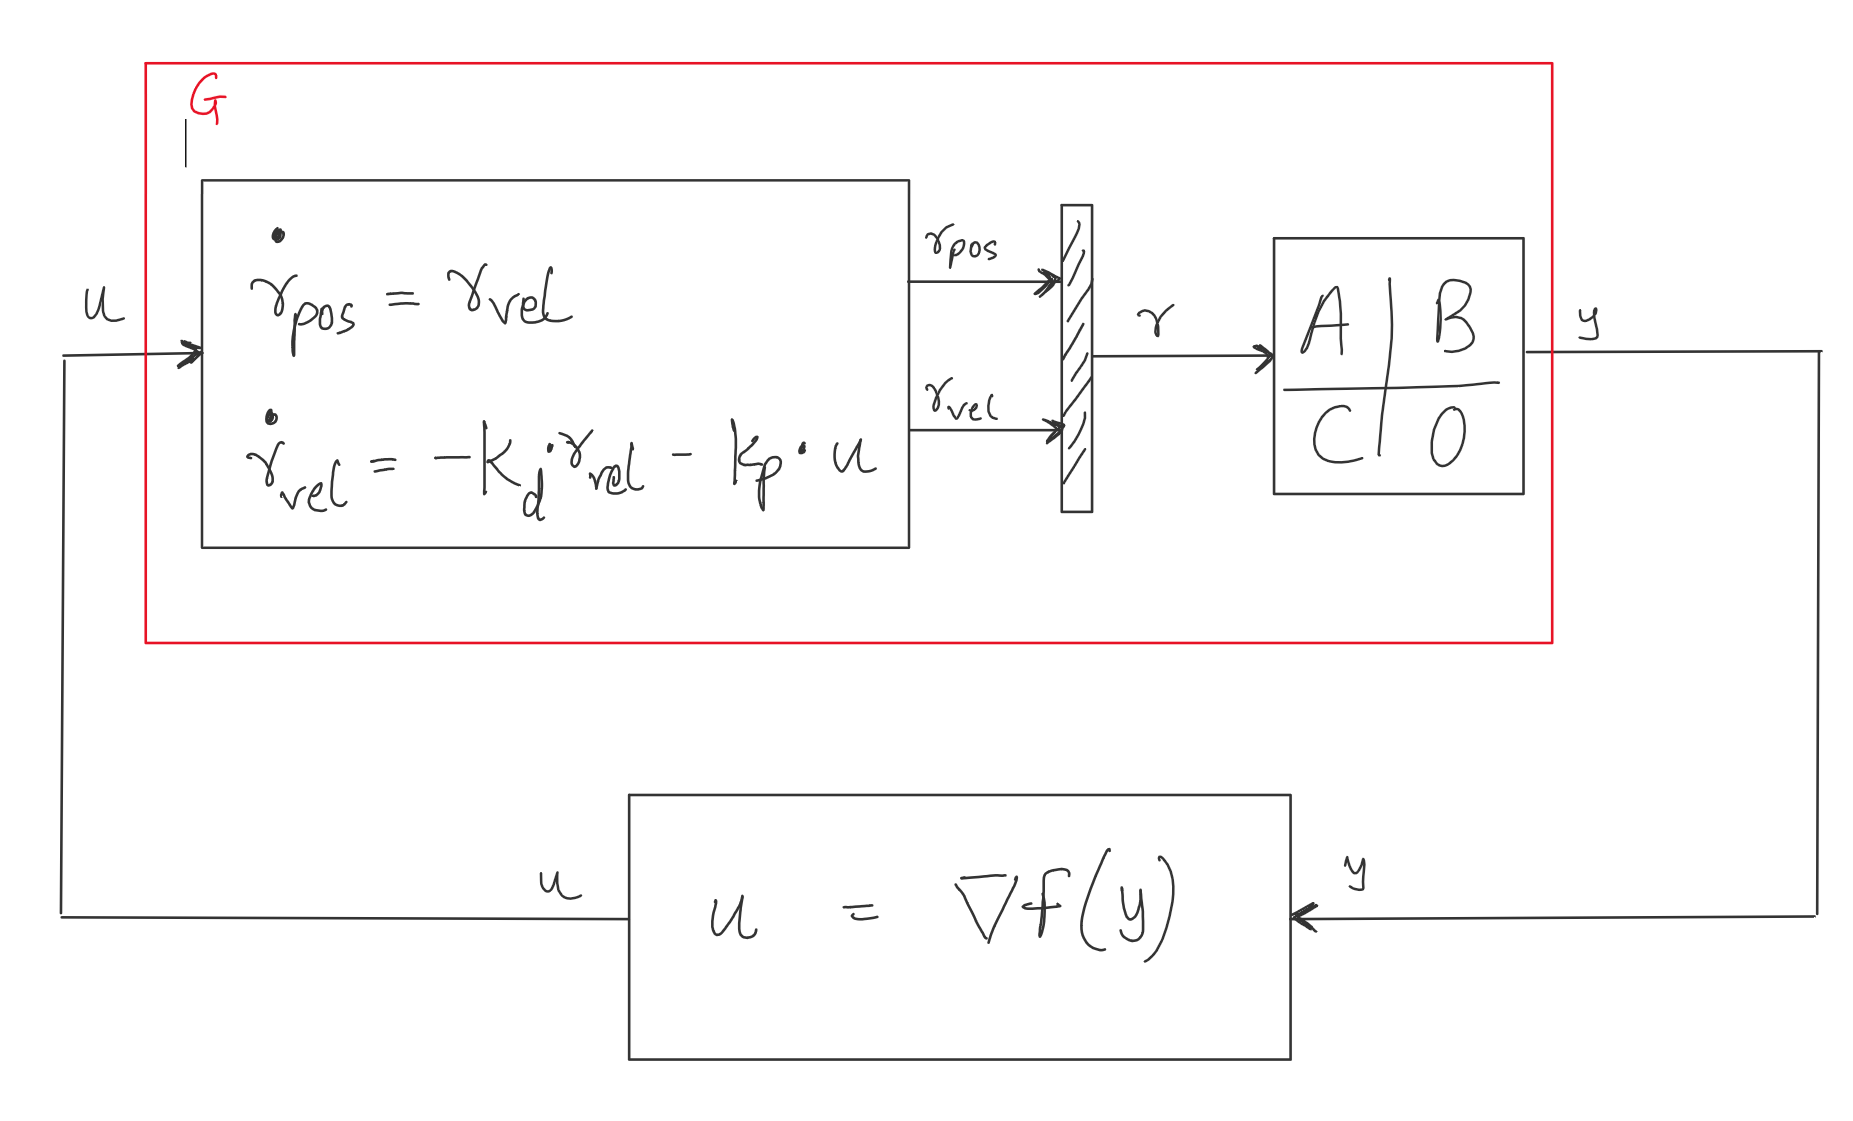
\includegraphics[width=8cm]{figures/Figure_IQC_paper.PNG}
		% This file was created by matlab2tikz.
%
%The latest updates can be retrieved from
%  http://www.mathworks.com/matlabcentral/fileexchange/22022-matlab2tikz-matlab2tikz
%where you can also make suggestions and rate matlab2tikz.
%
\definecolor{mycolor1}{rgb}{0.00000,1.00000,1.00000}%
%
\begin{tikzpicture}

\begin{axis}[%
width=2.321in,
height=2.266in,
at={(1in,2in)},
scale only axis,
xmin=1,
xmax=2.5,
xlabel style={font=\color{white!15!black}},
xlabel={$L$},
ymin=0,
ymax=0.5,
ylabel style={font=\color{white!15!black}},
ylabel={$\alpha$},
axis background/.style={fill=white},
title style={font=\bfseries},
title={},
legend style={legend cell align=left, align=left, draw=white!15!black}
]
\addplot [color=red, only marks, mark=o, mark options={solid, red}]
  table[row sep=crcr]{%
1	0.2520751953125\\
1.1	0.2520751953125\\
1.2	0.2520751953125\\
1.3	0.2520751953125\\
1.4	0.2197265625\\
1.5	0.1800537109375\\
1.6	0.1397705078125\\
1.7	0.0994873046875\\
1.8	0.0579833984375\\
1.9	0.0164794921875\\
2	-1\\
2.1	-1\\
2.2	-1\\
2.3	-1\\
2.4	-1\\
2.5	-1\\
2.6	-1\\
2.7	-1\\
2.8	-1\\
2.9	-1\\
3	-1\\
3.1	-1\\
3.2	-1\\
3.3	-1\\
3.4	-1\\
3.5	-1\\
3.6	-1\\
3.7	-1\\
3.8	-1\\
3.9	-1\\
4	-1\\
};
\addlegendentry{CC}

\addplot [color=green, only marks, mark=asterisk, mark options={solid, green}]
  table[row sep=crcr]{%
1	0.2520751953125\\
1.1	0.2520751953125\\
1.2	0.2520751953125\\
1.3	0.2520751953125\\
1.4	0.2197265625\\
1.5	0.1800537109375\\
1.6	0.1397705078125\\
1.7	0.0994873046875\\
1.8	0.0579833984375\\
1.9	0.0164794921875\\
2	-1\\
2.1	-1\\
2.2	-1\\
2.3	-1\\
2.4	-1\\
2.5	-1\\
2.6	-1\\
2.7	-1\\
2.8	-1\\
2.9	-1\\
3	-1\\
3.1	-1\\
3.2	-1\\
3.3	-1\\
3.4	-1\\
3.5	-1\\
3.6	-1\\
3.7	-1\\
3.8	-1\\
3.9	-1\\
4	-1\\
};
\addlegendentry{ZFb causal}

\addplot [color=blue, only marks, mark=o, mark options={solid, blue}]
  table[row sep=crcr]{%
1	0.2520751953125\\
1.1	0.2520751953125\\
1.2	0.2520751953125\\
1.3	0.2520751953125\\
1.4	0.2423095703125\\
1.5	0.208740234375\\
1.6	0.174560546875\\
1.7	0.1397705078125\\
1.8	0.1043701171875\\
1.9	0.068359375\\
2	0.0311279296875\\
2.1	-1\\
2.2	-1\\
2.3	-1\\
2.4	-1\\
2.5	-1\\
2.6	-1\\
2.7	-1\\
2.8	-1\\
2.9	-1\\
3	-1\\
3.1	-1\\
3.2	-1\\
3.3	-1\\
3.4	-1\\
3.5	-1\\
3.6	-1\\
3.7	-1\\
3.8	-1\\
3.9	-1\\
4	-1\\
};
\addlegendentry{ZFb anti causal}

\addplot [color=mycolor1, only marks, mark=o, mark options={solid, mycolor1}]
  table[row sep=crcr]{%
1	0.2520751953125\\
1.1	0.2520751953125\\
1.2	0.2520751953125\\
1.3	0.2520751953125\\
1.4	0.2520751953125\\
1.5	0.2520751953125\\
1.6	0.2520751953125\\
1.7	0.238037109375\\
1.8	0.2142333984375\\
1.9	0.1885986328125\\
2	0.1611328125\\
2.1	0.1324462890625\\
2.2	0.1019287109375\\
2.3	0.0701904296875\\
2.4	0.0360107421875\\
2.5	-1\\
2.6	-1\\
2.7	-1\\
2.8	-1\\
2.9	-1\\
3	-1\\
3.1	-1\\
3.2	-1\\
3.3	-1\\
3.4	-1\\
3.5	-1\\
3.6	-1\\
3.7	-1\\
3.8	-1\\
3.9	-1\\
4	-1\\
};
\addlegendentry{ZFb non causal}

\addplot [color=black, only marks, mark=asterisk, mark options={solid, black}]
  table[row sep=crcr]{%
1	0.252381023686084\\
1.1	0.285030034676752\\
1.2	0.319444587967699\\
1.3	0.322120595821607\\
1.4	0.30294136645159\\
1.5	0.282662461122388\\
1.6	0.261201184778797\\
1.7	0.238470096600161\\
1.8	0.214377762177947\\
1.9	0.188829987346274\\
2	0.161731674331652\\
2.1	0.132989449419385\\
2.2	0.102515199007407\\
2.3	0.0702306031940527\\
2.4	0.0360726564236493\\
2.5	-1.11022302462516e-16\\
2.6	-0.0380003387049317\\
2.7	-0.0779064749243448\\
2.8	-0.119656383851905\\
2.9	-0.163144853458106\\
3	-0.208223620537594\\
3.1	-0.254705253392262\\
3.2	-0.302370714578469\\
3.3	-0.350979820177716\\
3.4	-0.400283236115395\\
3.5	-0.450034410796233\\
3.6	-0.500000000000001\\
3.7	-0.549967803542309\\
3.8	-0.599751818251013\\
3.9	-0.649194534678147\\
4	-0.698166954229536\\
};
\addlegendentry{Example field}

\end{axis}
\end{tikzpicture}%
		\caption{Robustness for $G(s)=5\frac{(s-1)}{s(s^2+s+25)}$ and $m=1$}
		\centering
		\label{fig:benefit_of_non_causal_multipliers}
	\end{figure}	
\end{frame}
%%%%%%%%%%%%%%%%%%%%%%%%%%%%%%%%%%%%%%%%%%%%%%%%%%%%%%%%%%%%%%%%%%%%%
\begin{frame}{Ongoing work and next steps }
	\begin{block}{Forseeable extensions}
	\begin{itemize}
		\item Source-seeking with formation control with a leader (Grounded Laplacians) (\textbf{Tested and seems to work} )
		\item LPV vehicle models
		\item Extend the full block ZF multipliers to the $\alpha$- IQC case
		\item Controller synthesis with DK-iteration?
		\item Mean squared stability analysis with MJLS
	\end{itemize}
\end{block}
\end{frame}
%%%%%%%%%%%%%%%%%%%%%%%%%%%%%%%%%%%%%%%%%%%%%%%%%%%%%%%%%%%%%%%%%%%%%
\begin{frame}{References}
	\begin{itemize}
		\item[1] C.  Scherer,  “Dissipativity  and  integral  quadratic  constraints,  tailoredcomputational robustness tests for complex interconnections.” [Online].Available: https://arxiv.org/pdf/2105.07401
		\item[2]  M.  Fazlyab,  A.  Ribeiro,  M. Morari,  and  V.  M.  Preciado,  “Analysis  ofoptimization algorithms via integral quadratic constraints: Nonstronglyconvex  problems,”SIAM  Journal  on  Optimization,  vol.  28,  no.  3,  pp.2654–2689, 2018.
		\item[3]  A.  Datar,  P.  Paulsen,  and  H.  Werner,  “Flocking  towards  the  source:Indoor experiments with quadrotors,” in2020 European Control Con-ference (ECC).    IEEE, 5/12/2020 - 5/15/2020, pp. 1638–1643.
		\item[4]  A.  Attallah,  A.  Datar,  and  H.  Werner,  “Flocking  of  linear  parametervarying  agents:  Source  seeking  application  with  underwater  vehicles,”IFAC-PapersOnLine, vol. 53, no. 2, pp. 7305–7311, 2020.		
	\end{itemize}
\end{frame}
%%%%%%%%%%%%%%%%%%%%%%%%%%%%%%%%%%%%%%%%%%%%%%%%%%%%%%%%%%%%%%%%%%%%%
\begin{frame}{References}
	\begin{itemize}		
		\item[5]  L.  Lessard,  B.  Recht,  and  A.  Packard,  “Analysis  and  design  of  opti-mization  algorithms  via  integral  quadratic  constraints,”SIAM  Journalon Optimization, vol. 26, no. 1, pp. 57–95, 2016.
		\item[6]  B.  Hu  and  P.  Seiler,  “Exponential  decay  rate  conditions  for  uncertainlinear systems using integral quadratic constraints,”IEEE Transactionson Automatic Control, vol. 61, no. 11, pp. 3631–3637, 2016.
		\item[7]  R. A. Freeman, “Noncausal zames-falb multipliers for tighter estimatesof  exponential  convergence  rates,”  in2018  Annual  American  ControlConference (ACC).    IEEE, 6/27/2018 - 6/29/2018, pp. 2984–2989.
		\item[8]  J.   Veenman   and   C.   W.   Scherer,   “Stability   analysis   with   integralquadratic  constraints:  A  dissipativity  based  proof,”  in52nd  IEEEConference on Decision and Control, 2013, pp. 3770–3775.
	\end{itemize}
\end{frame}
%%%%%%%%%%%%%%%%%%%%%%%%%%%%%%%%%%%%%%%%%%%%%%%%%%%%%%%%%%%%%%%%%%%%%
\begin{frame}{References}
	\begin{itemize}		
		\item[9]  J.    Zhang,    P.    Seiler,    and    J.    Carrasco,    “Noncausal    fir    zames-falb  multiplier  search  for  exponential  convergence  rate.”  [Online].Available: https://arxiv.org/pdf/1902.09473
	\end{itemize}
\end{frame}
%%%%%%%%%%%%%%%%%%%%%%%%%%%%%%%%%%%%%%%%%%%%%%%%%%%%%%%%%%%%%%%%%%%%%
\begin{frame}{}
\begin{center}
    \huge{Thank you}
\end{center}
\end{frame}
%%%%%%%%%%%%%%%%%%%%%%%%%%%%%%%%%%%%%%%%%%%%%%%%%%%%%%%%%%%%%%%%%%%%%
%%%%%%%%%%%%%%%%%%%%%%%%%%%%%%%%%%%%%%%%%%%%%%%%%%%%%%%%%%%%%%%%%%%%%
%\begin{frame}{Abstracting to a Mathematical Problem}	
%\begin{block}{Problem Statement:}
%Design distributed control algorithms for large networks of mobile robots such that the group shows a desirable behavior.
%\end{block}
%\begin{itemize}
%	\item Desirable behaviors we consider:
%	\begin{itemize}
%		\item Consensus and/or Formation stabilization
%		\item Flocking with/without source seeking
%	\end{itemize}	
%	\item Complexity in solving the problem can stem through:
%	\begin{itemize}
%		\item Complicated dynamics of individual agents
%		\item Commplicated Interconnection structure and intractible design algorithms for large networks
%	\end{itemize}
%\end{itemize}
%\end{frame}
%%%%%%%%%%%%%%%%%%%%%%%%%%%%%%%%%%%%%%%%%%%%%%%%%%%%%%%%%%%%%%%%%%%%%
%\begin{frame}{Approaching the problem: Divide and Conquer}
%\begin{block}{Available literature on}
%\begin{itemize}
%	\item Control of single complex agent dynamics (e.g LPV, control of differetially flat systems, dynamic inversion) 
%	\item Distributed control of large networks of "simple" agent dynamics (e.g single and double intergrators) -> Consensus and Flocking algorithms
%\end{itemize}
%\end{block}	
%\begin{block}{Consider as building blocks}
%\begin{itemize}
%	\item Closed-loop system $G_{\textnormal{cl}}$ with some guaranteed performance measure such as the induced $\mathcal{L}_2-\mathcal{L}_2$ or  $\mathcal{L}_2-\mathcal{L}_{\infty}$ norms
%	\item Consensus or Flocking algorithms for "simple" systems
%\end{itemize}
%\end{block}
%\end{frame}
%%%%%%%%%%%%%%%%%%%%%%%%%%%%%%%%%%%%%%%%%%%%%%%%%%%%%%%%%%%%%%%%%%%%%
\end{document}

